\documentclass[10pt,a4paper]{article}

\usepackage[margin=1.5cm,bottom=1.8cm,footskip=0.7cm]{geometry}
\usepackage[T1]{fontenc}
\usepackage{lmodern}
\usepackage{amsmath,amssymb}
\usepackage{booktabs,tabularx,array}
\usepackage{makecell}
\usepackage{graphicx}
\usepackage{float}
\usepackage{enumitem}
\usepackage{titlesec}
\usepackage{fancyhdr}
\usepackage{lastpage}
\usepackage{xcolor}
\usepackage{tikz}
\usetikzlibrary{positioning,fit,backgrounds,arrows.meta,calc}
\usepackage[labelformat=empty,font=small,labelfont=bf,textfont=bf,justification=raggedright,singlelinecheck=false,skip=2pt]{caption}
\usepackage[colorlinks=true,linkcolor=red,urlcolor=blue]{hyperref}

% Headings with a rule underneath, as in the Assignment 1 report
\titleformat{\section}{\normalsize\bfseries}{}{0pt}{}[\titlerule]
\titleformat{\subsection}{\normalsize\bfseries}{}{0pt}{}
\titlespacing*{\section}{0pt}{6pt}{3pt}
\titlespacing*{\subsection}{0pt}{5pt}{1pt}
\setcounter{secnumdepth}{0}

\setlist[itemize]{leftmargin=*,itemsep=0pt,topsep=1pt,parsep=0pt}
\setlength{\parindent}{0pt}
\setlength{\parskip}{1pt}
\setlength{\tabcolsep}{3pt}
\setlength{\textfloatsep}{4pt}
\setlength{\floatsep}{4pt}
\setlength{\intextsep}{4pt}

\pagestyle{fancy}
\fancyhf{}
\renewcommand{\headrulewidth}{0pt}
\renewcommand{\footrulewidth}{0.4pt}
\fancyfoot[L]{\small Ali Haider (24280058)}
\fancyfoot[C]{\small AI651 Assignment 2}
\fancyfoot[R]{\small Page \thepage\ of \pageref{LastPage}}

% Question 1 table columns
\newcolumntype{L}{>{\raggedright\arraybackslash}X}
\newcolumntype{P}[1]{>{\raggedright\arraybackslash}p{#1}}
% Question 2: mean (seed 0, seed 1) on two lines
\newcommand{\ms}[3]{\makecell{#1\\[-2pt]\tiny(#2, #3)}}
\newcommand{\sci}[2]{$#1{\times}10^{#2}$}
\newcommand{\q}[1]{\textbf{#1}}
\newcommand{\todo}[1]{\textcolor{red}{[#1]}}

\begin{document}

\begin{center}
{\bfseries Lahore University of Management Sciences}\\
School of Science and Engineering, Department of Artificial Intelligence\\
{\bfseries AI651 -- Deep Learning for Space, Time and Graphs}, Fall 2026\\[3pt]
{\bfseries Assignment 2: Report for Questions 1 and 2}\\
Ali Haider (Roll No: 24280058) \quad GitHub: \todo{add the public PA2 repository link}
\end{center}

\section{Question 1: River forecasting proposal}

Every 10 minutes the system forecasts the level one hour ahead at S1--S4, as a range (10\%, 50\%, 90\%) plus the chance of passing the warning level. The design asks, for each station: \emph{what decides its level in one hour, where is that information at forecast time, and what path carries it to the forecast?}

\subsection{1. Architecture diagram}
Each source is put on one 10-minute clock (block 2) and turned into tokens: one reading from one source at one step, stored as 64 numbers (block 3). Each token reads its own and upstream tokens (block 4), one query per station collects what that station needs (block 5), and block 6 returns levels in metres (Figure 1).

\begin{figure}[H]
\caption{Figure 1: Forecasting system. Grey labels are tensor shapes: $B$ = batch, 36 = past 10-min steps (6 h), 6 = next-hour steps, 64 = token size, 330 = tokens. Dashed: fixed river mask and training-only loss. The output row reads right to left.}
\centering
\hyphenpenalty=10000 \exhyphenpenalty=10000
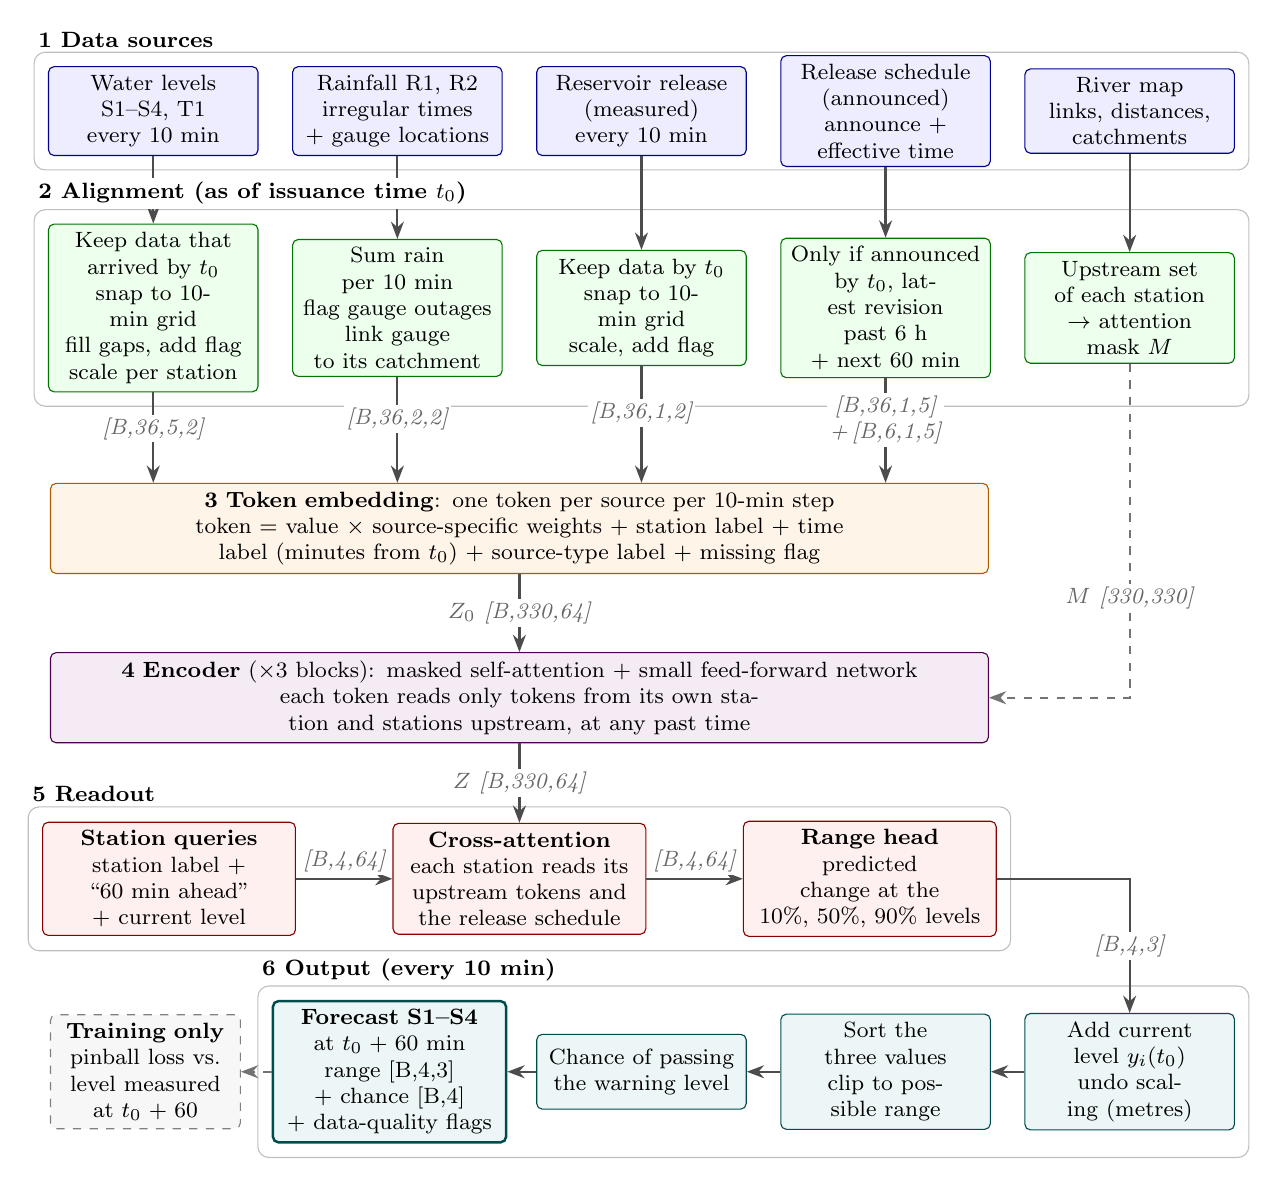
\begin{tikzpicture}[
  font=\fontsize{8}{9.5}\selectfont,
  box/.style={draw, rounded corners=2pt, align=center, minimum height=0.95cm, inner sep=3pt},
  src/.style={box, fill=blue!7, draw=blue!55!black, text width=2.45cm},
  pre/.style={box, fill=green!7, draw=green!45!black, text width=2.45cm},
  emb/.style={box, fill=orange!9, draw=orange!70!black},
  enc/.style={box, fill=violet!8, draw=violet!60!black},
  dec/.style={box, fill=red!6, draw=red!55!black, text width=3.0cm},
  outb/.style={box, fill=teal!7, draw=teal!60!black, text width=2.45cm},
  shp/.style={font=\fontsize{8}{9.5}\selectfont\itshape, text=black!60, fill=white, inner sep=1pt},
  arr/.style={-{Stealth[length=2.2mm]}, thick, black!70},
  dsh/.style={-{Stealth[length=2.2mm]}, thick, dashed, black!55},
  grp/.style={draw=black!25, rounded corners=4pt, inner sep=5pt},
  tag/.style={font=\fontsize{8}{9.5}\selectfont\bfseries, anchor=south west, inner sep=1.5pt}
]
% ---- row 1: sources
\node[src] (s1) at (0,0)    {Water levels\\S1--S4, T1\\every 10 min};
\node[src] (s2) at (3.1,0)  {Rainfall R1, R2\\irregular times\\+ gauge locations};
\node[src] (s3) at (6.2,0)  {Reservoir release\\(measured)\\every 10 min};
\node[src] (s4) at (9.3,0)  {Release schedule\\(announced)\\announce + effective time};
\node[src] (s5) at (12.4,0) {River map\\links, distances,\\catchments};
% ---- row 2: alignment
\node[pre] (a1) at (0,-2.5)    {Keep data that\\arrived by $t_0$\\snap to 10-min grid\\fill gaps, add flag\\scale per station};
\node[pre] (a2) at (3.1,-2.5)  {Sum rain per 10 min\\flag gauge outages\\link gauge\\to its catchment};
\node[pre] (a3) at (6.2,-2.5)  {Keep data by $t_0$\\snap to 10-min grid\\scale, add flag};
\node[pre] (a4) at (9.3,-2.5)  {Only if announced\\by $t_0$, latest revision\\past 6 h\\+ next 60 min};
\node[pre] (a5) at (12.4,-2.5) {Upstream set\\of each station\\$\to$ attention mask $M$};
\foreach \i in {1,...,5} \draw[arr] (s\i) -- (a\i);
% ---- row 3: embedding
\node[emb, text width=11.7cm] (e) at (4.65,-5.3) {\textbf{3 Token embedding}: one token per source per 10-min step\\
token = value $\times$ source-specific weights $+$ station label $+$ time label (minutes from $t_0$) $+$ source-type label $+$ missing flag};
\draw[arr] (a1) -- node[shp, pos=0.4]{[B,36,5,2]} (a1 |- e.north);
\draw[arr] (a2) -- node[shp, pos=0.4]{[B,36,2,2]} (a2 |- e.north);
\draw[arr] (a3) -- node[shp, pos=0.4]{[B,36,1,2]} (a3 |- e.north);
\draw[arr] (a4) -- node[shp, pos=0.4, align=center]{[B,36,1,5]\\+\,[B,6,1,5]} (a4 |- e.north);
% ---- row 4: encoder
\node[enc, text width=11.7cm] (n) at (4.65,-7.45) {\textbf{4 Encoder} ($\times$3 blocks): masked self-attention $+$ small feed-forward network\\
each token reads only tokens from its own station and stations upstream, at any past time};
\draw[arr] (e) -- node[shp]{$Z_0$ [B,330,64]} (n);
\draw[dsh] (a5.south) |- node[shp, pos=0.35]{$M$ [330,330]} (n.east);
% ---- row 5: readout
\node[dec] (q) at (0.2,-9.75)  {\textbf{Station queries}\\station label $+$ ``60 min ahead'' $+$ current level};
\node[dec] (x) at (4.65,-9.75) {\textbf{Cross-attention}\\each station reads its upstream tokens and the release schedule};
\node[dec] (h) at (9.1,-9.75)  {\textbf{Range head}\\predicted change at the\\10\%, 50\%, 90\% levels};
\draw[arr] (n) -- node[shp]{$Z$ [B,330,64]} (x);
\draw[arr] (q) -- node[shp, above=1pt]{[B,4,64]} (x);
\draw[arr] (x) -- node[shp, above=1pt]{[B,4,64]} (h);
% ---- row 6: output (right to left)
\node[outb] (o1) at (12.4,-12.2) {Add current level $y_i(t_0)$\\undo scaling (metres)};
\node[outb] (o2) at (9.3,-12.2)  {Sort the three values\\clip to possible range};
\node[outb] (o3) at (6.2,-12.2)  {Chance of passing\\the warning level};
\node[outb, text width=2.75cm, line width=0.9pt] (o4) at (3.0,-12.2) {\textbf{Forecast S1--S4}\\at $t_0+60$ min\\range [B,4,3]\\+ chance [B,4]\\+ data-quality flags};
\draw[arr] (h.east) -| node[shp, pos=0.75]{[B,4,3]} (o1.north);
\draw[arr] (o1) -- (o2);
\draw[arr] (o2) -- (o3);
\draw[arr] (o3) -- (o4);
\node[box, dashed, draw=black!50, fill=black!3, text width=2.2cm] (l) at (-0.1,-12.2) {\textbf{Training only}\\pinball loss vs.\ level measured at $t_0+60$};
\draw[dsh] (o4) -- (l);
% ---- group frames
\begin{scope}[on background layer]
\node[grp, fit=(s1)(s5)] (g1) {}; \node[tag] at (g1.north west) {1 Data sources};
\node[grp, fit=(a1)(a5)] (g2) {};
\node[grp, fit=(q)(h)] (g5) {};   \node[tag] at (g5.north west) {5 Readout};
\node[grp, fit=(o4)(o1)] (g6) {}; \node[tag] at (g6.north west) {6 Output (every 10 min)};
\end{scope}
\node[tag, fill=white] at (g2.north west) {2 Alignment (as of issuance time $t_0$)};
\end{tikzpicture}
\end{figure}

\subsection{2. Assumptions}
\textbf{Supplied facts:} 10-min levels at S1--S4 and T1; rain at R1, R2 with times and locations; measured releases and schedules with announcement and effective times; river links and distances. \textbf{Not supplied:} travel times and unmonitored-tributary data. Future rain and levels are never available.
\begin{itemize}
\item \textbf{A1 Record:} 3+ years of data including flood seasons. \emph{Why:} the authority already runs these stations. \emph{Effect:} $\sim$157,000 training samples; split by time (train, then validate, then test on the latest year).
\item \textbf{A2 Clock:} one time zone; a rain value is rain since the last report. \emph{Why:} normal for one telemetry system. \emph{Effect:} all sources fit one grid.
\item \textbf{A3 Delays:} most readings arrive within 10 min, some up to 1 h late; arrival times are logged. \emph{Why:} typical of radio or mobile links. \emph{Effect:} only data that has arrived is used, in training too.
\item \textbf{A4 Bad values:} gaps are mostly under 1 h; out-of-range values count as missing. \emph{Why:} typical sensor behaviour. \emph{Effect:} every input has a missing flag.
\item \textbf{A5 Gauges:} R1 drains near S1 and R2 into the unmonitored tributary. \emph{Why:} their positions on the site map. \emph{Effect:} R1 feeds S1--S4; R2 feeds S3, S4 and is the only clue to the unmonitored inflow.
\item \textbf{A6 Travel time:} reservoir to S4 takes 15 min (high flow) to 4 h (low flow), never over 5 h; rain reaches the river within 4 h. \emph{Why:} flood waves move faster in a full river. \emph{Effect:} a 6 h history covers it; lags are learned, not fixed.
\item \textbf{A7 Downstream only:} within an hour a station is affected only by itself and what is upstream (no backwater). \emph{Why:} a hillside river flowing fast in one direction. \emph{Effect:} the attention mask.
\item \textbf{A8 Releases:} measured releases are accurate; schedules can be revised and are usually followed; all revisions are archived. \emph{Why:} dam gates are metered, and operators react to conditions. \emph{Effect:} measured and scheduled releases are separate token types.
\item \textbf{A9 Stable river:} no new dams or channel changes. \emph{Why:} the brief mentions none. \emph{Effect:} one model for the whole record, retrained every few months for slow change.
\item \textbf{A10 Warning levels:} each station has one. \emph{Why:} standard for flood authorities. \emph{Effect:} the system can report the chance of passing it.
\end{itemize}

\subsection{3. Forecasting task and data specification}
\textbf{Issuance} $t_0$: every 10 min, using only data arrived by $t_0$. \textbf{History:} 36 steps, $k=-35..0$ (slot $k$ is time $t_0+10k$ min). \textbf{Horizon:} the level at $t_0+60$; next-hour release schedules are known future inputs ($k=+1..+6$). Later releases cannot arrive in time. \textbf{Batch} $B$: issuance times processed together ($B=1$ live).

\begin{table}[!htb]
\caption{Table 1: Inputs and outputs (flag = 1 if missing or filled in)}
\scriptsize
\begin{tabularx}{\textwidth}{@{}P{2.3cm}P{1.45cm}LP{2.6cm}@{}}
\toprule
Item & Shape & Axes & Time coverage \\
\midrule
Water levels & [B,36,5,2] & batch; lag; S1, S2, S3, S4, T1; (level, flag) & $t_0-350$ to $t_0$ min \\
Rainfall & [B,36,2,2] & batch; lag; R1, R2; (mm in slot, flag) & $t_0-350$ to $t_0$ \\
Release, measured & [B,36,1,2] & batch; lag; dam; (release, flag) & $t_0-350$ to $t_0$ \\
Schedule, past & [B,36,1,5] & batch; lag; dam; (scheduled, change, announcement age, measured$-$scheduled, flag) & as known at $t_0$ \\
Schedule, next hour & [B,6,1,5] & batch; lag $+1..+6$; dam; same (measured$-$scheduled $=0$) & $t_0+10$ to $t_0+60$ \\
River mask $M$ & [330,330] & token; token; 0 allowed, $-\infty$ blocked & fixed \\
\midrule
Output range & [B,4,3] & batch; S1--S4; 10/50/90\% level (m) & at $t_0+60$ \\
Warning chance & [B,4] & batch; S1--S4 & at $t_0+60$ \\
Target (training) & [B,4] + flag & batch; S1--S4; measured level & at $t_0+60$ \\
\bottomrule
\end{tabularx}
\end{table}

\textbf{Alignment.} Each slot holds the latest level, the total rain and the mean release in that 10 min. Schedules go in the slot of their effective time, using the latest revision \emph{announced} by $t_0$. Upstream data is \emph{not} shifted by a guessed travel time; the model sees the full window and learns the lag. Location enters as a station label. \textbf{Available at $t_0$:} readings that arrived by $t_0$, schedules announced by $t_0$, the river map. \textbf{Not available:} future rain and levels, late readings, later revisions, unmonitored inflow.

\subsection{4. Model computations and design justification}
\textbf{Notation:} source $n$, lag $k$, features $x_{n,k}$, missing flag $m_{n,k}$, token size $d=64$, station $i$, current level $y_i(t_0)$, range level $\tau\in\{0.1,0.5,0.9\}$.
{\small\begin{align*}
&\text{Token:} && e_{n,k} = W_{\text{type}(n)}x_{n,k} + E_{\text{node}}[n] + E_{\text{lag}}[k] + E_{\text{src}}[\text{type}(n)] + m_{n,k}e_{\text{miss}}\\
&\text{Encoder (}\times 3\text{):} && Z' = Z + \text{softmax}\big(QK^\top/\sqrt{16} + M\big)V,\quad Z \leftarrow Z' + \text{FFN}(Z')\\
&\text{Readout:} && q_i = E_{\text{node}}[S_i] + E_{\text{lag}}[+6] + w\,y_i(t_0),\quad \Delta_i = \text{MLP}\big(\text{CrossAtt}(q_i, Z; M_i)\big)\in\mathbb{R}^3\\
&\text{Forecast:} && \hat y_i^{\tau} = \mu_i + \sigma_i\big(\tilde y_i(t_0) + \Delta_i^{\tau}\big), \text{ then sorted and clipped}\\
&\text{Loss:} && \mathcal{L} = \tfrac{1}{N}\textstyle\sum_{b,i} v_{b,i}\,(1+\lambda\mathbf{1}[y_{b,i}>w_i])\sum_\tau \rho_\tau(y_{b,i}-\hat y^{\tau}_{b,i}),\quad \rho_\tau(u)=\max(\tau u,(\tau-1)u)
\end{align*}}
$M=0$ only where the read token is from the same or an upstream station (A7). $v_{b,i}=0$ for missing targets. Weight $\lambda$ stops rare floods being drowned out (layer norms and the 4 heads are omitted).

\textbf{Why these choices.}
\begin{itemize}
\item \textbf{A token per step} lets the model point at ``S2, 40 min ago''; the right lag changes with flow, and attention picks it from the current state.
\item \textbf{Attention, not small convolutions:} any upstream source is reachable in one step (the notebook showed local blocks failing beyond their reach), and 330 tokens is cheap.
\item \textbf{The mask} adds the one sure physical fact and blocks false links (e.g.\ S4 ``predicting'' S1 because both react to rain).
\item \textbf{Predicting the change} starts from ``no change'', which is already strong over one hour.
\item \textbf{A range, not one value:} with missing information, squared error averages the possible futures and flattens flood peaks.
\end{itemize}
\textbf{How sources reach each forecast.} Releases reach every station, most strongly S1. Upstream levels and T1 reach the stations below them. R1 reaches S1--S4. R2 and S3's own recent rise are the only signs of the unmonitored tributary at S3, S4. \textbf{Physics (fixed):} river links, flow direction, window length, gauge catchments. \textbf{Learned:} travel times at each flow, wave growth or shrinkage, the rain-to-rise response, schedule reliability, range width. \textbf{Check:} beat persistence, and the 10--90\% range should hold the truth about 80\% of the time. S4 should barely attend to next-hour releases, since that water cannot reach it in time.

\subsection{5. Operation and exceptional conditions}
\begin{itemize}
\item \textbf{(i) Missing:} fill with the last value and set the flag, so the model leans on other stations. Training hides random readings and short outages. Missing targets are skipped in the loss.
\item \textbf{(ii) Delayed:} only data \emph{arrived} by $t_0$ is used; a late reading counts as missing now and is used next cycle. Training uses arrival times, and the forecast lists late inputs.
\item \textbf{(iii) Announced releases:} one token per slot $t_0+10..t_0+60$, using the latest revision announced by $t_0$. Later revisions would leak future information.
\item \textbf{(iv) Schedule vs.\ actual:} the past 6 h show both values and their gap, so the model learns how far to trust the schedule. The new measurement is used 10 min later; large gaps raise an operator alert.
\item \textbf{Feasibility:} about 0.21 M parameters and about 0.1 billion multiply-adds per forecast, so well under a second on a CPU. Training is offline (under an hour on one GPU), with retraining every few months. If a run fails, a persistence forecast is published, marked stale.
\end{itemize}

\subsection{6. Uncertainty, limitations, and additional information}
\begin{itemize}
\item \textbf{U1 Unmonitored tributary:} S3, S4 can rise unseen. Response: R2 and S3's trend, with wider ranges. Unresolved: inflow without rain at R2.
\item \textbf{U2 Changing travel times:} a fixed lag would be wrong exactly in floods. Response: attention picks the lag from the current flow. Unresolved: floods larger than any in the record.
\item \textbf{U3 Future rain:} can raise levels within the hour before it is measured. Response: ranges widen after heavy recent rain. Unresolved without rain forecasts (I3).
\item \textbf{U4 Unannounced releases:} change S1 within the hour. Response: picked up at the next run, 10 min later. Unresolved: the first forecast after one.
\item \textbf{U5 Rare floods:} few examples, so peaks may be under-predicted. Response: flood weighting and clipping. Unresolved: levels never seen before.
\item \textbf{U6 River change and only two gauges:} the level--flow link drifts, and local storms are missed. Response: retraining and wider ranges.
\end{itemize}

\begin{table}[H]
\caption{Table 2: Information requested from the authority}
\scriptsize
\begin{tabularx}{\textwidth}{@{}P{4.4cm}LP{4.2cm}@{}}
\toprule
Request & How it helps & Usable without it? \\
\midrule
I1 Gauge on the unmonitored tributary & removes the S3/S4 blind spot (U1) & yes, with wider ranges \\
I2 Schedule revisions with announcement times & honest training (A8) & yes, but over-trusts schedules \\
I3 Rain forecasts or radar & covers next-hour rain (U3) & yes, past rain only \\
I4 Arrival-time logs & realistic delays (A3) & yes, with assumed delays \\
I5 Warning level per station & warning chance (A10) & partly: ranges only \\
I6 Travel-time studies & checks the 6 h window and lags (A6) & yes, relies on A6 \\
\bottomrule
\end{tabularx}
\end{table}

\clearpage
\section{Question 2: Motion or Memory?}

A ConvLSTM video model (model A) predicts the next 5 frames of Moving MNIST from 5 frames. To see whether it learned \emph{how digits move} or only \emph{what training videos look like}, I mirror ($M$), rotate by $90^\circ$ ($R$) or speed up ($2\times$, $3\times$) the test clips. $C_T$ is the \textbf{consistency gap}: how much the forecast changes if the clip is transformed before predicting instead of after (0 means fully consistent). $E_T$ is the error on the transformed clip. All numbers are on the 1,000 test videos (lower is better), and learned models are shown as mean (seed 0, seed 1). All training (Adam, learning rate $10^{-3}$, batch 32, 30 epochs) and all timings ran on one NVIDIA RTX PRO 6000 GPU.

\subsection{1. Setup}

\noindent\begin{minipage}[t]{0.47\textwidth}
\captionof{table}{Table 3: transformation and window checks}
\centering\scriptsize
\begin{tabular}{lll}
\toprule
 & Check & Expected = mine \\
\midrule
(a) & largest $|M(M(x)) - x|$ & 0 (exact) \\
(b) & largest $|R^4(x) - x|$ & 0 (exact) \\
(c) & largest $|MRM(x) - R^{-1}(x)|$ & 0 (exact) \\
(d) & bright pixel of $M(p)$ & (7, 10, 43) \\
(e) & bright pixel of $R(p)$ & (7, 43, 10) \\
(f) & $1\times$ input / target frames & 1--5 / 6--10 \\
(g) & $2\times$ input / target frames & 1, 3, 5, 7, 9 / 11, 13, 15, 17, 19 \\
(h) & $3\times$ input / target frames & 1, 4, 7, 10, 13 / 16, 19 \\
\bottomrule
\end{tabular}
\end{minipage}\hfill
\begin{minipage}[t]{0.51\textwidth}
\captionof{figure}{Figure 2: direction (a) and speed (b) of motion in the first 50 training videos}
\centering
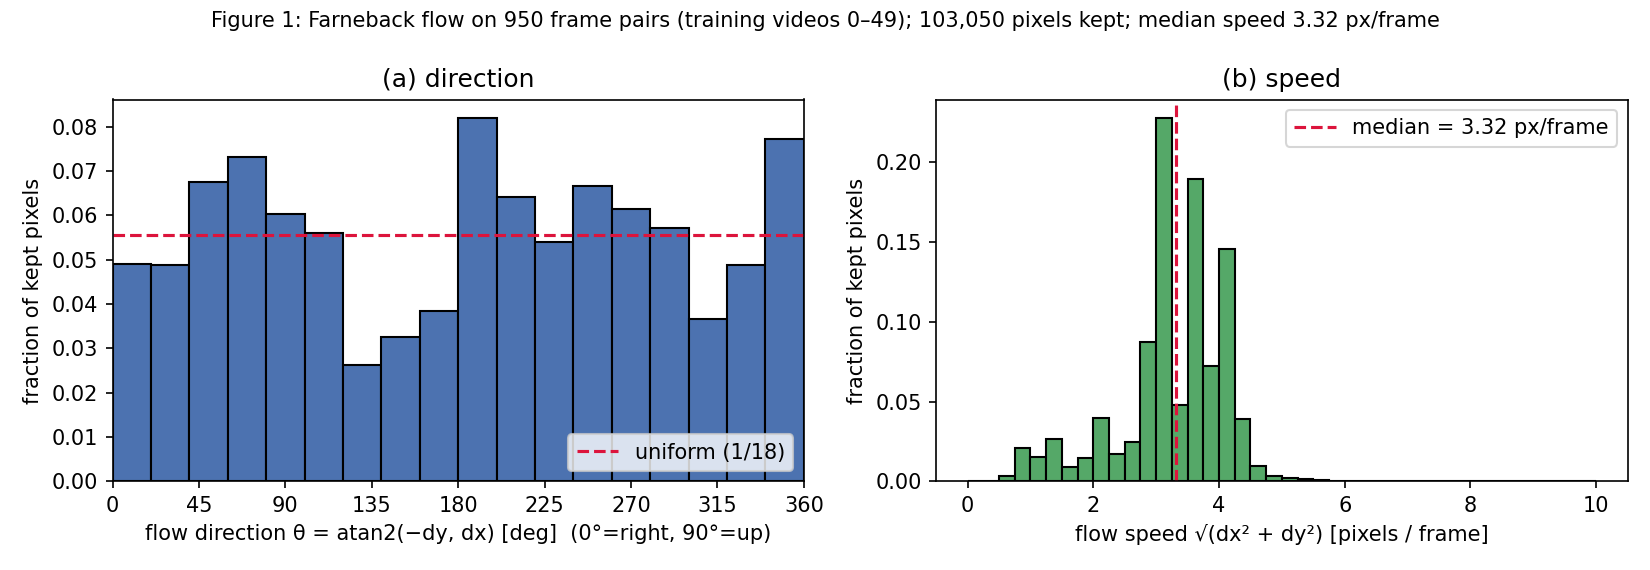
\includegraphics[width=\linewidth]{../Question2/figures/figure1_flow.png}
\end{minipage}

\q{Q2.1 Are mirrored and rotated motions already familiar? What speeds do $1\times$, $2\times$, $3\times$ mean? Could overlaps bias this?}
\begin{itemize}
  \item Mirroring flips the direction histogram left to right, and rotating shifts it by $90^\circ$; a flat histogram would not change. Ours is close to flat (bins 0.026--0.082 around 0.056) with no favoured direction, which is what about 100 digit paths give by chance. So \textbf{mirrored and rotated motion is familiar}; only the digits' look is new.
  \item The typical speed is \textbf{3.3 px/frame} (90\% below 4.1). So $2\times$ is about \textbf{6.6} and $3\times$ about \textbf{10 px/frame}, faster than almost anything seen in training.
  \item Where digits overlap, two motions blend into one slower one. That adds slow values, not a favoured direction, so the answer holds.
\end{itemize}

\q{Q2.2 What does each transformation change?} Mirror and rotation keep the motion but change how the digits look (rotation more, since upright strokes turn sideways). Speed-up keeps the digits but changes the motion. So $M$ and $R$ test appearance and speed tests motion, one factor at a time.

\subsection{2. The Baseline: Model A}

\q{Q2.3 Model A's reach.} The model folds each $4 \times 4$ pixel patch into one grid cell, so one cell is 4 px. Each $3 \times 3$ convolution passes information one cell, and the two layers in a row give 2 cells, i.e.\ \textbf{8 px per step} (in each direction). The other parts (folding, $1 \times 1$ layers, gates) move nothing. A gradient check gives the same 8 px. Model A has 480,784 parameters.

\begin{table}[H]
\caption{Table 4: model A against the two simple predictors ($1\times$)}
\centering\scriptsize
\begin{tabular}{lccccccr}
\toprule
Model & MSE$_1$ & MSE$_2$ & MSE$_3$ & MSE$_4$ & MSE$_5$ & $E^{(5)}$ (mean of 5) & Params \\
\midrule
Blank & 0.0426 & 0.0426 & 0.0426 & 0.0425 & 0.0425 & 0.0426 & 0 \\
Copy-last & 0.0492 & 0.0604 & 0.0669 & 0.0708 & 0.0732 & 0.0641 & 0 \\
Model A & \ms{0.0171}{0.0175}{0.0168} & \ms{0.0205}{0.0208}{0.0201} & \ms{0.0227}{0.0230}{0.0224} & \ms{0.0244}{0.0247}{0.0242} & \ms{0.0261}{0.0263}{0.0259} & \ms{0.0222}{0.0225}{0.0219} & 480,784 \\
\bottomrule
\end{tabular}
\end{table}

\q{Q2.4 How does model A compare, and what happens when digits overlap?}
\begin{itemize}
  \item Model A's error (0.0222) is about half of Blank's (0.0426) and a third of Copy-last's (0.0641), at every horizon. Copy-last is worse than Blank because a digit in the wrong place is counted twice.
  \item Its error grows from 0.0171 to 0.0261 over the 5 frames (+52\%), because from frame 6 it reads its own blurry output.
  \item When digits overlap it predicts \textbf{one blob that never splits again} (Figure 3, all three videos).
\end{itemize}

\q{Q2.5 Pre-registered prediction:}
\begin{enumerate}[leftmargin=*,itemsep=0pt,topsep=1pt,parsep=0pt]
  \item \textbf{Mirror test:} Model A will \textbf{fail}. The motion looks normal, but mirrored digits (2, 3, 5, 6) look unfamiliar. The model never saw flipped digits during training.
  \item \textbf{Rotation test ($90^\circ$):} Model A will do \textbf{worse than on the mirror test}. Turning digits sideways changes their shape more than flipping them does.
  \item \textbf{Speed:} $1\times$: works well. Digits move about 3.3 px per frame, under the model's 8 px limit. $2\times$: starts to degrade. Digits move about 6.6 px per frame, and the fastest ones exceed 8 px. $3\times$: breaks down. Digits move about 10--14 px per frame, beyond what the model can track in one step. Expect blurring, frozen digits, or ghost copies.
\end{enumerate}

\subsection{3. Testing the Baseline}

\noindent\begin{minipage}[t]{0.33\textwidth}
\captionof{figure}{Figure 3: inputs, model A predictions and truth for test videos 0--2 (digits overlap in all three)}
\centering
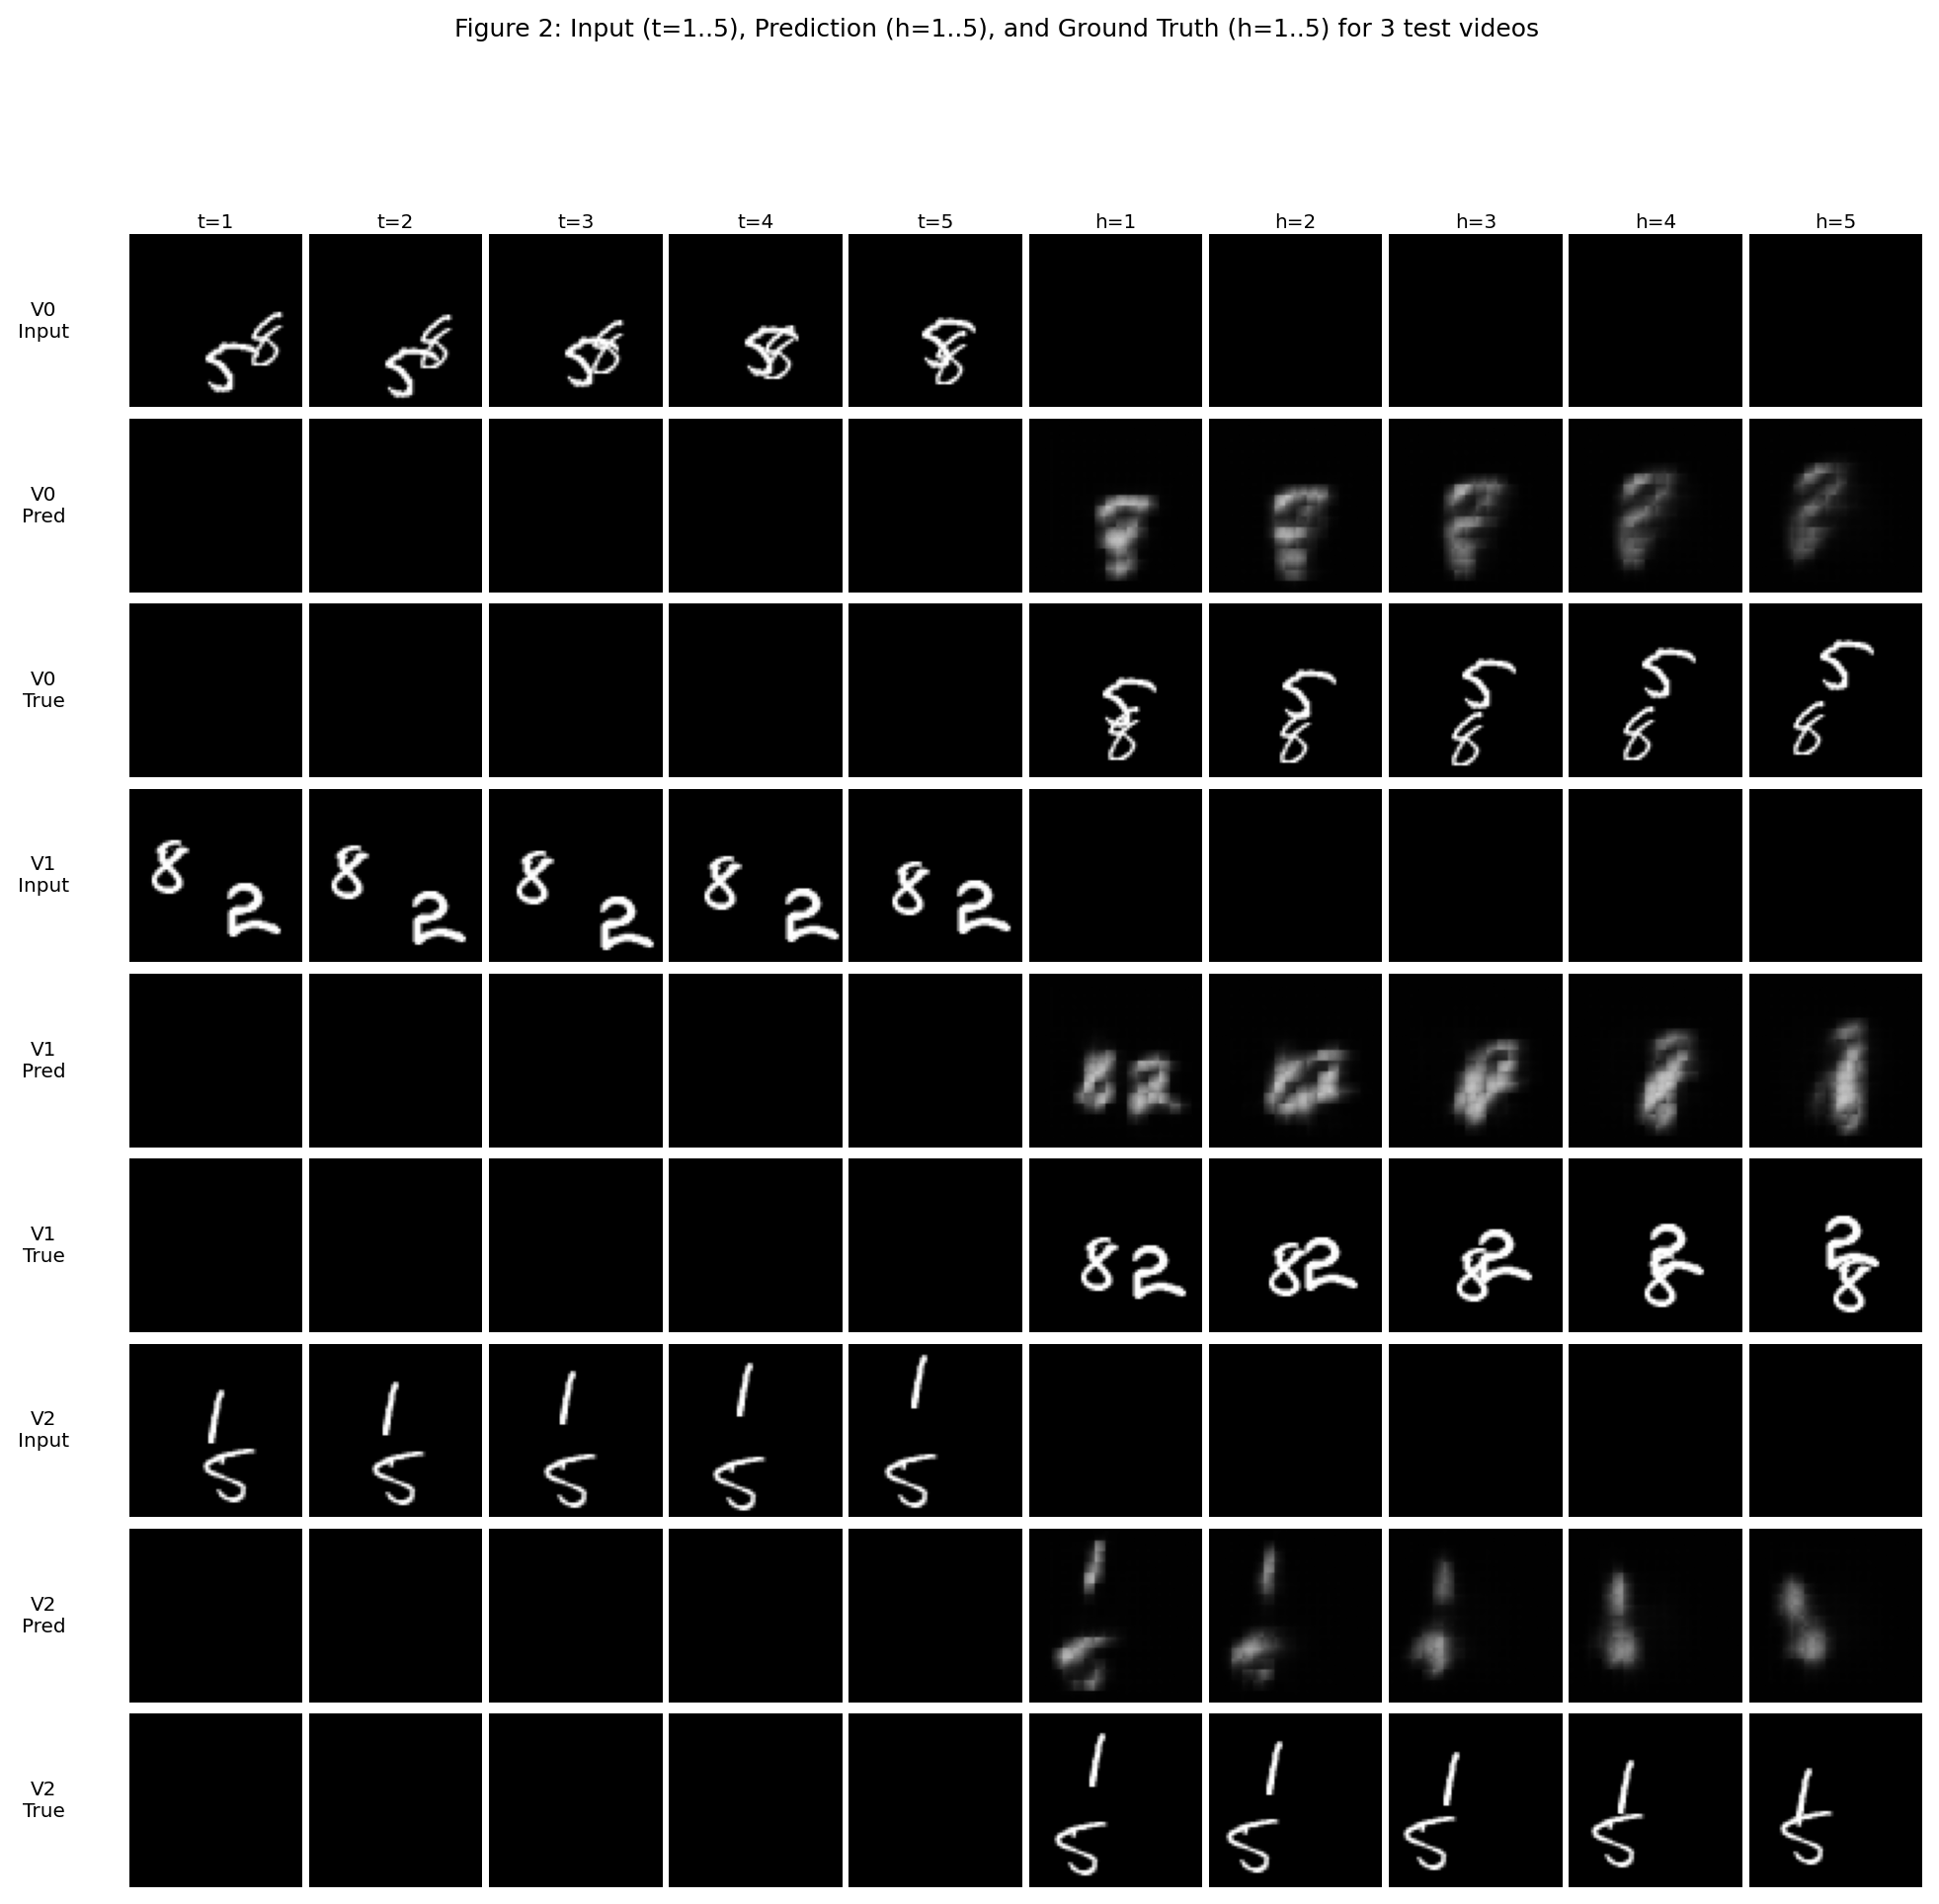
\includegraphics[width=\linewidth]{../Question2/figures/figure2_predictions.png}
\end{minipage}\hfill
\begin{minipage}[t]{0.64\textwidth}
\captionof{table}{Table 5: mirror and rotation ($1\times$)}
\centering\scriptsize
\begin{tabular}{lccccc}
\toprule
Model & $E^{(5)}$ & $C_M$ & $E_M$ & $C_R$ & $E_R$ \\
\midrule
Blank & 0.0426 & 0 & 0.0426 & 0 & 0.0426 \\
Copy-last & 0.0641 & 0 & 0.0641 & 0 & 0.0641 \\
Model A & \ms{0.0222}{0.0225}{0.0219} & \ms{0.00186}{0.00161}{0.00211} & \ms{0.0228}{0.0230}{0.0225} & \ms{0.00298}{0.00268}{0.00329} & \ms{0.0239}{0.0240}{0.0238} \\
\bottomrule
\end{tabular}
\end{minipage}

\begin{figure}[H]
\caption{Figure 4: model A (seed 0) on the videos with the largest $C_M$ (499, 329) and $C_R$ (279, 733). Rows: clip and prediction; transformed clip and truth; prediction on the transformed clip; prediction transformed afterwards. GIFs in \texttt{gifs/}}
\centering
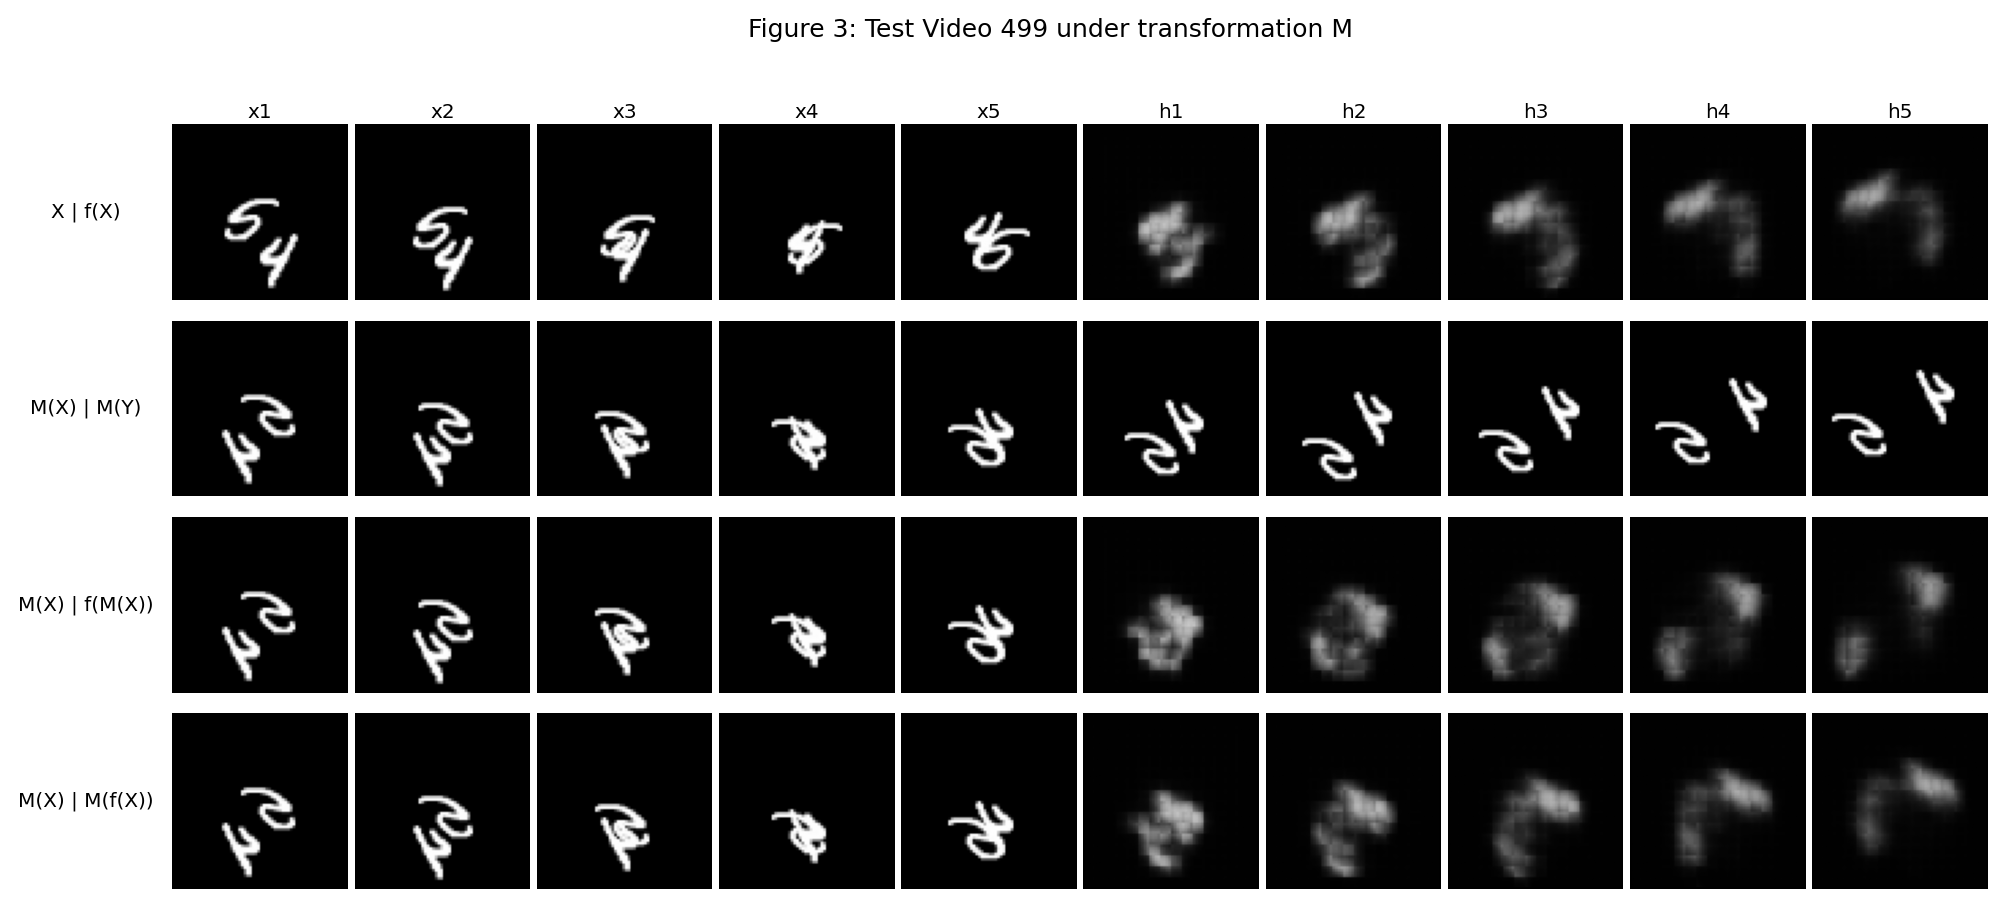
\includegraphics[width=0.37\textwidth]{../Question2/figures/figure3_M_top1_video499.png}\hspace{4pt}
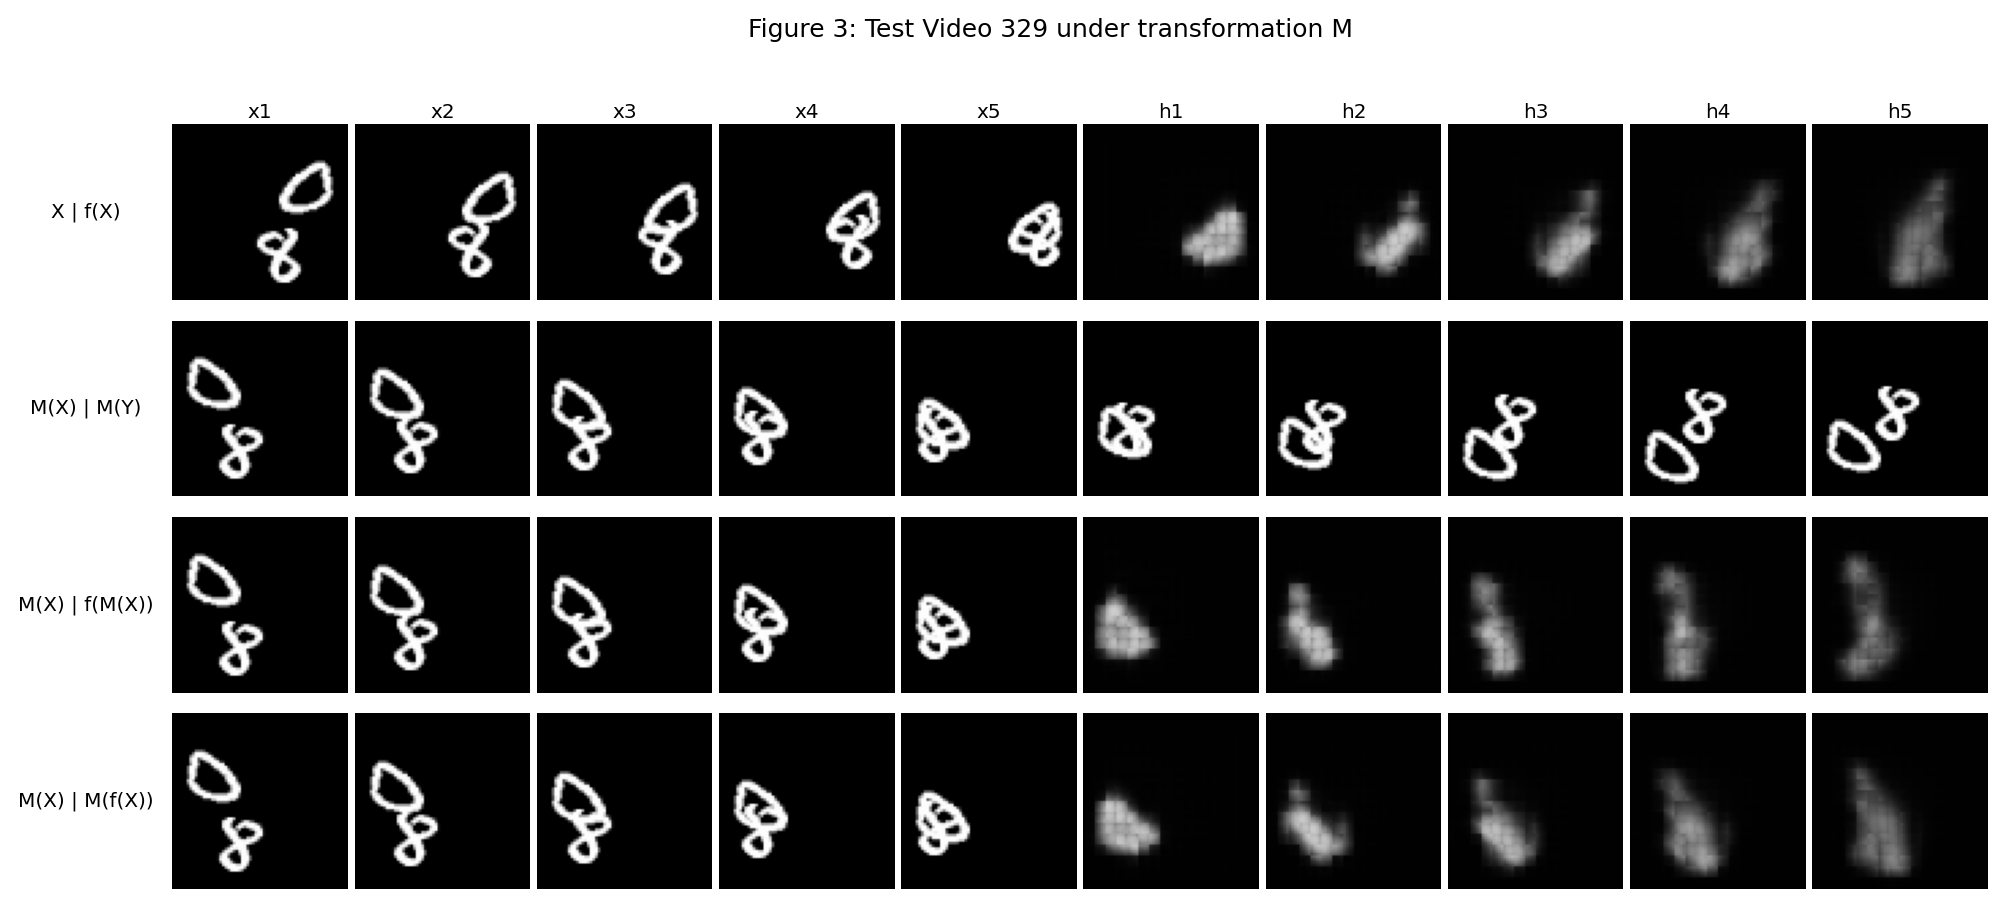
\includegraphics[width=0.37\textwidth]{../Question2/figures/figure3_M_top2_video329.png}\\[2pt]
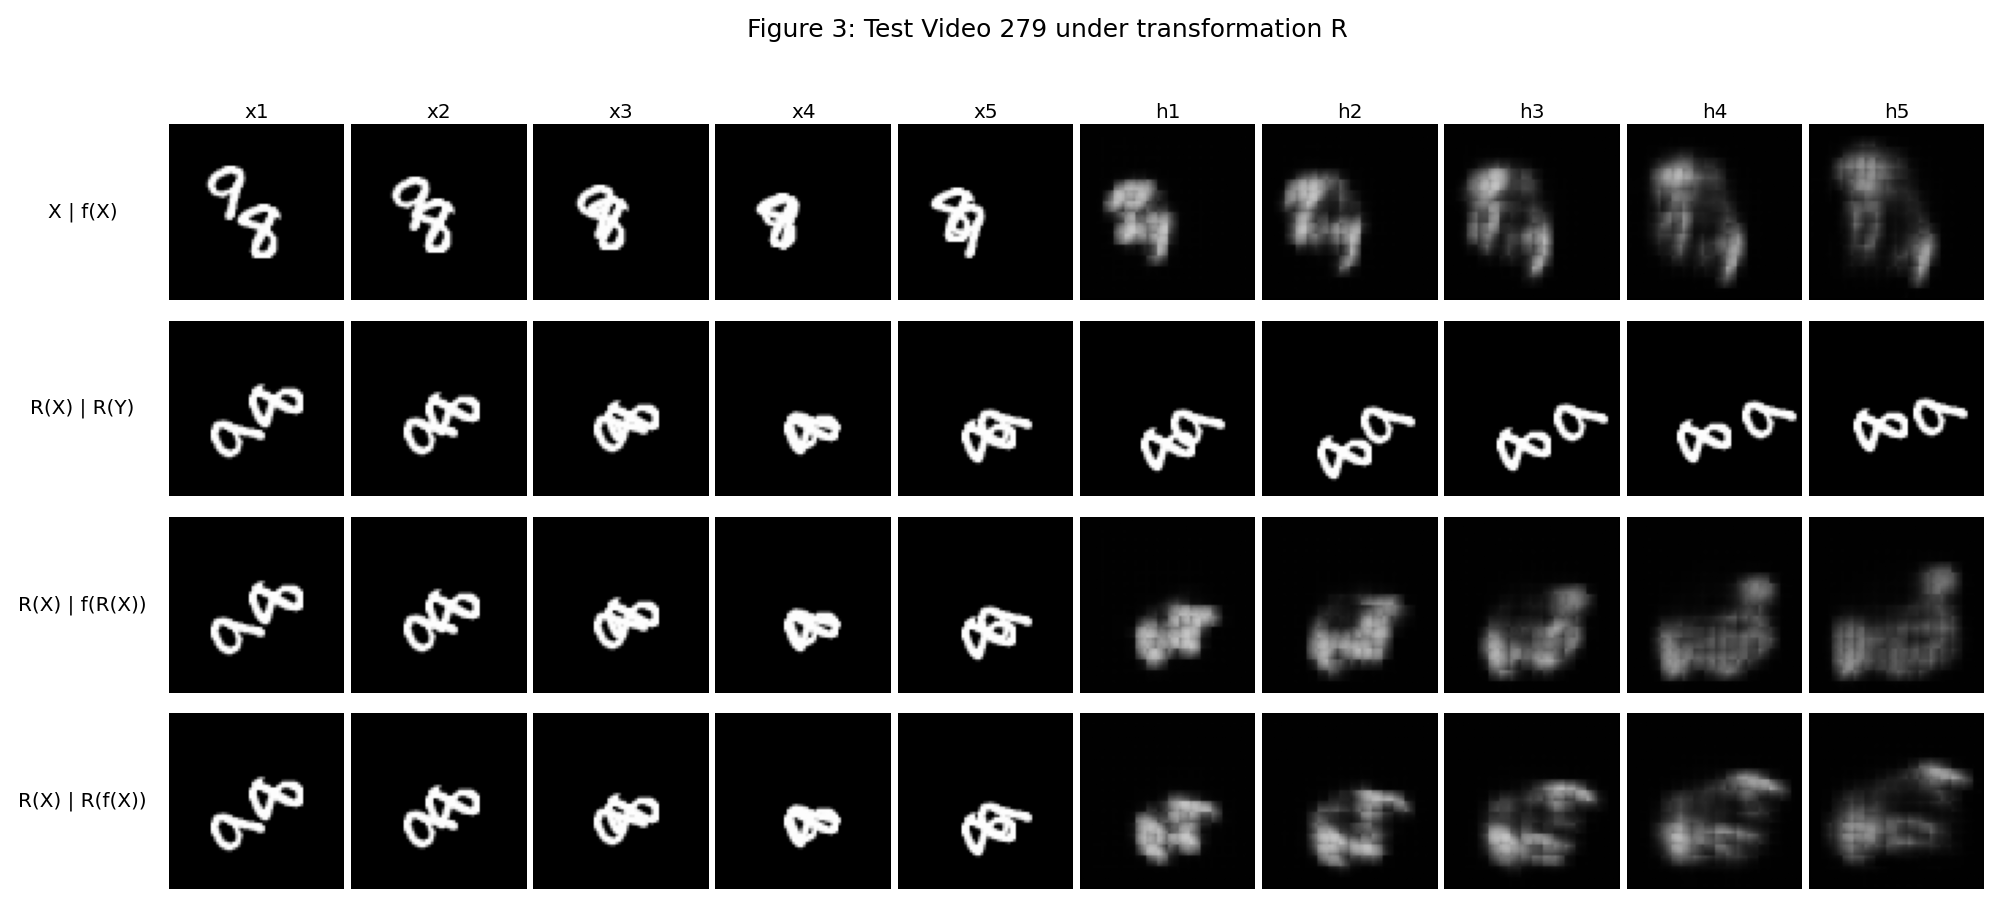
\includegraphics[width=0.37\textwidth]{../Question2/figures/figure3_R_top1_video279.png}\hspace{4pt}
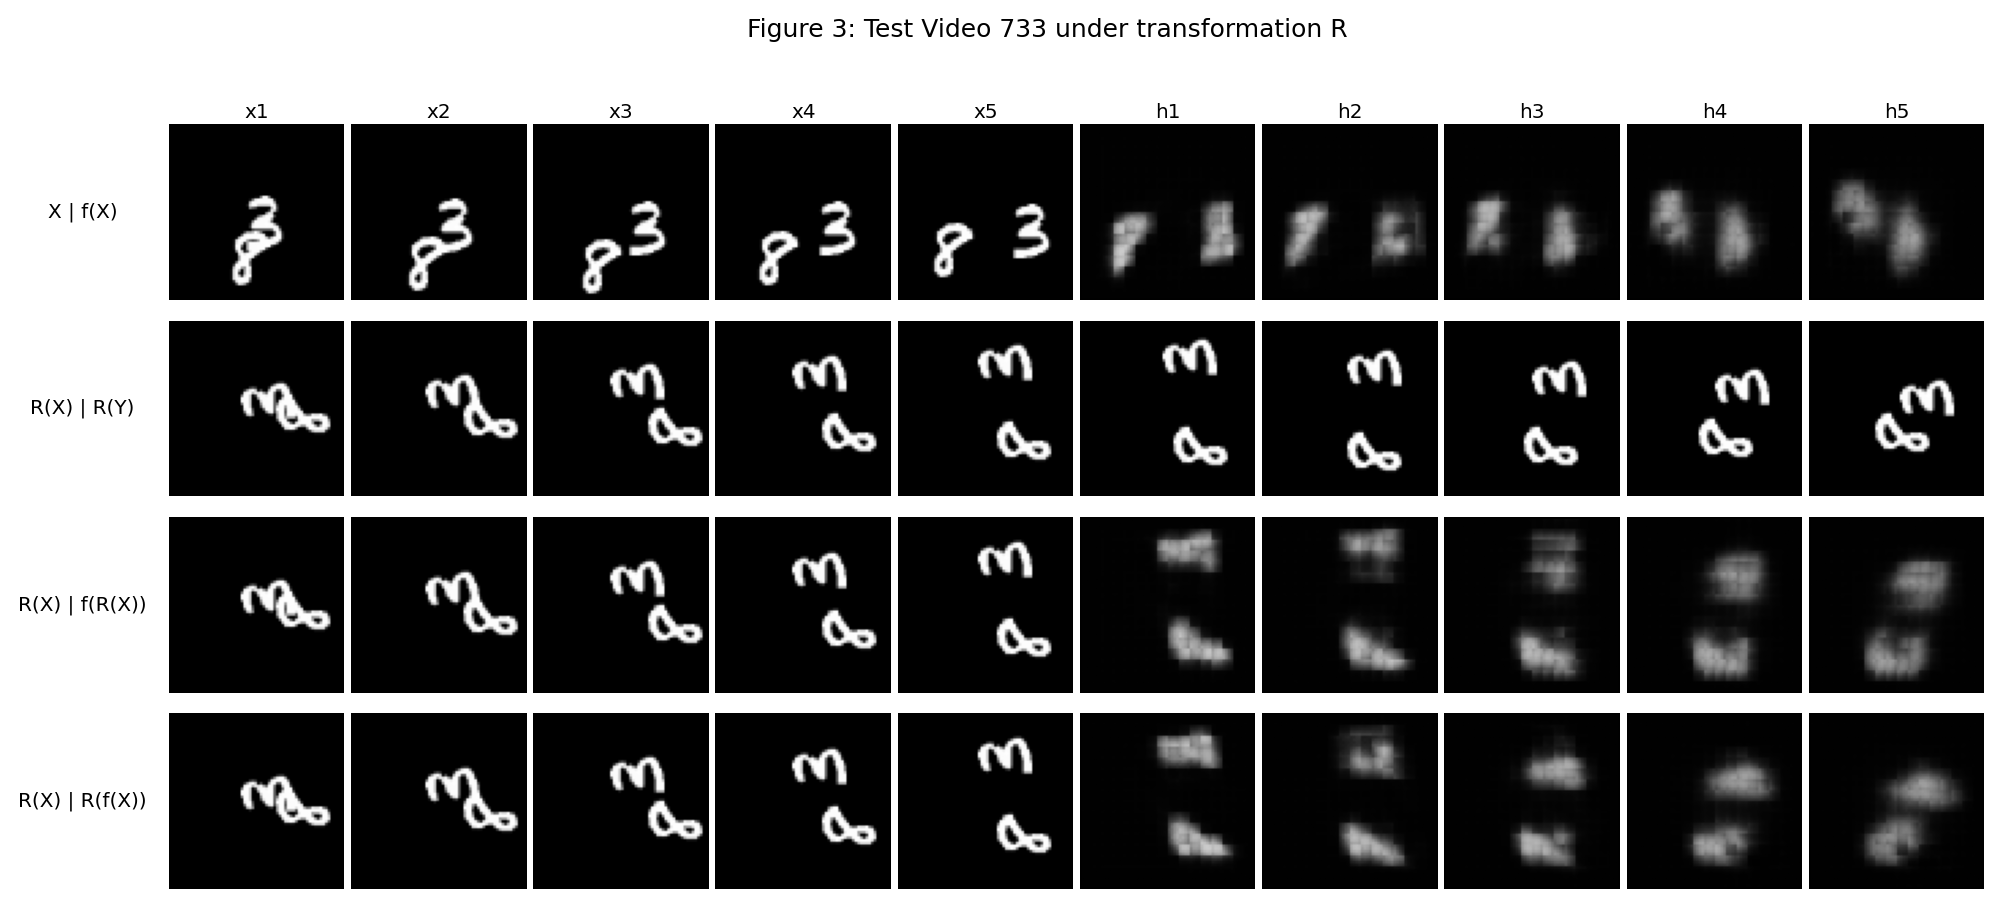
\includegraphics[width=0.37\textwidth]{../Question2/figures/figure3_R_top2_video733.png}
\end{figure}

\q{Q2.6 Why must $E_T$ be reported next to $C_T$?} Blank and Copy-last have $C = 0$, since flipping an empty or copied frame changes nothing, yet they know no motion and their error is about twice model A's. So a small gap alone can hide a useless model: the collapsed D seed 0 (Section 4) has the smallest gap of any learned model (\sci{2.68}{-7}) while predicting a plain grey frame. $E_T$ shows whether the gap matters: model A's $C_M$ (0.00186) is three times its real error increase (0.0006).

\q{Q2.7 One video where rows 3 and 4 disagree.} Video 499 under $M$: a 5 and a 4 cross and then separate. On the mirrored clip (row 3) the model splits them into \textbf{two blobs moving apart}, close to the truth. On the upright clip (row 4) it follows only the 4, and \textbf{the other digit gets lost} as a fading tail. Same motion, different story, depending only on how the digits look.

\q{Q2.8 Is rotation harder than mirroring?} Yes, mildly: rotation adds 8\% to the error and mirroring 3\% ($C_R$ 0.00298 against $C_M$ 0.00186, Table 5). The cause is appearance, not motion: both motions are familiar (Q2.1), but rotation turns upright strokes sideways. Model B, trained on flipped and rotated digits, removes both increases (Table 7).

\begin{table}[H]
\caption{Table 6: model A at faster speeds}
\centering\scriptsize
\begin{tabular}{lccccc}
\toprule
Model & $E^{(2)}$ $1\times$ & $E^{(2)}$ $2\times$ & $E^{(2)}$ $3\times$ & $E^{(5)}$ $1\times$ & $E^{(5)}$ $2\times$ \\
\midrule
Blank & 0.0426 & 0.0425 & 0.0426 & 0.0426 & 0.0425 \\
Copy-last & 0.0548 & 0.0661 & 0.0703 & 0.0641 & 0.0719 \\
Model A & \ms{0.0188}{0.0192}{0.0185} & \ms{0.0447}{0.0435}{0.0459} & \ms{0.0519}{0.0509}{0.0529} & \ms{0.0222}{0.0225}{0.0219} & \ms{0.0492}{0.0476}{0.0509} \\
\bottomrule
\end{tabular}
\end{table}

\noindent\begin{minipage}[t]{0.49\textwidth}
\captionof{figure}{Figure 5: per-video $C_M$ and $C_R$ of model A (seed 0), Figure 4 videos marked}
\centering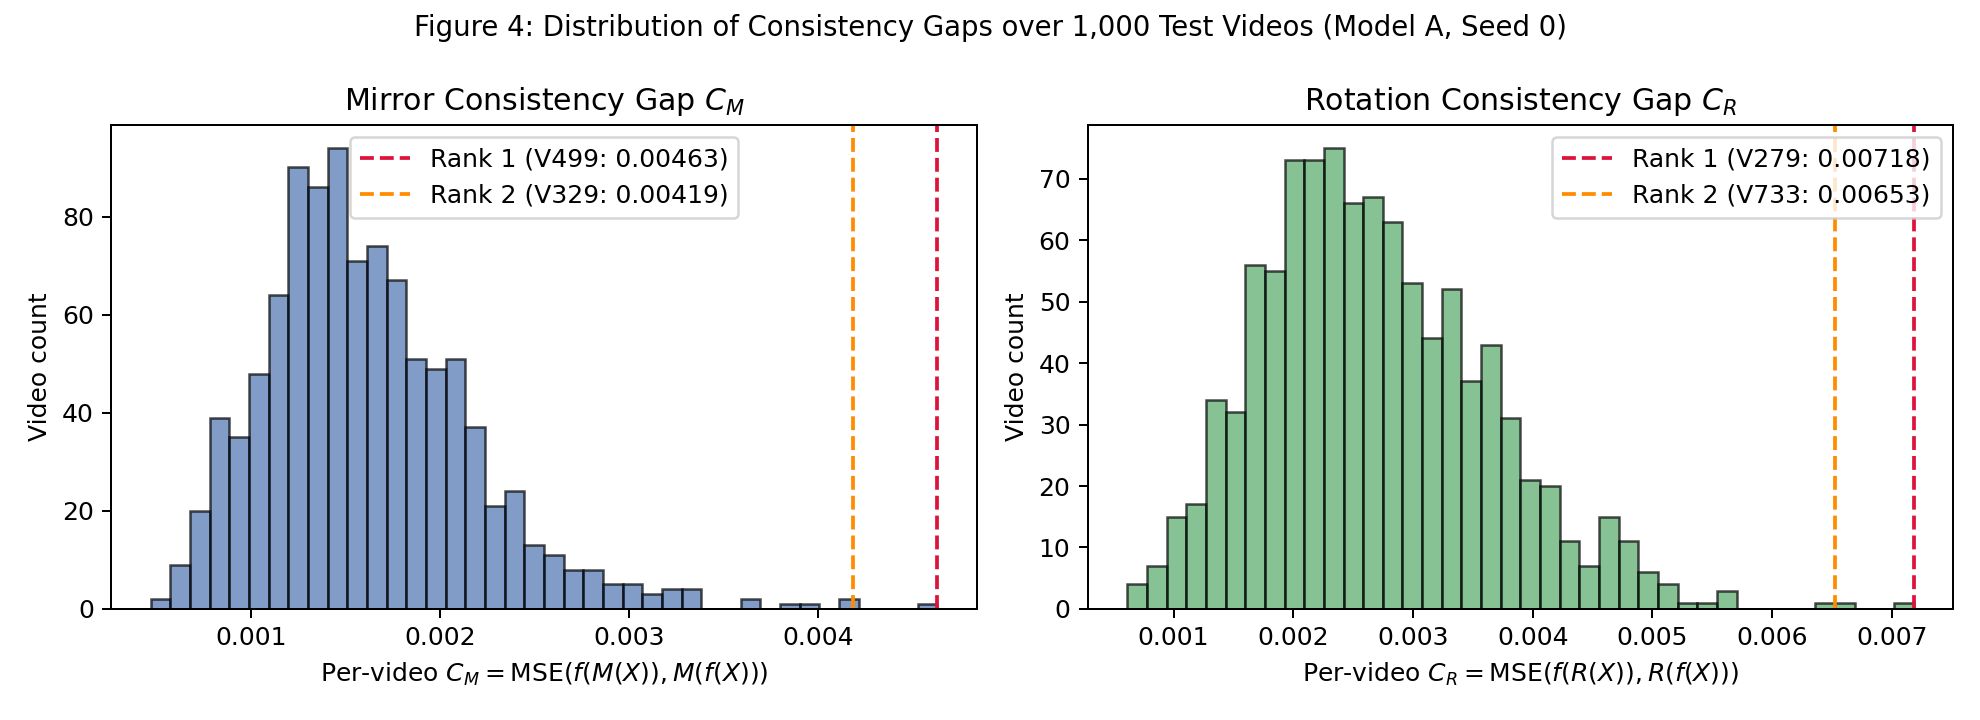
\includegraphics[width=\linewidth]{../Question2/figures/figure4_consistency_histograms.png}
\end{minipage}\hfill
\begin{minipage}[t]{0.49\textwidth}
\captionof{figure}{Figure 6: video 38 at $1\times$, $2\times$, $3\times$: inputs, two predictions (model A, seed 0), two true frames}
\centering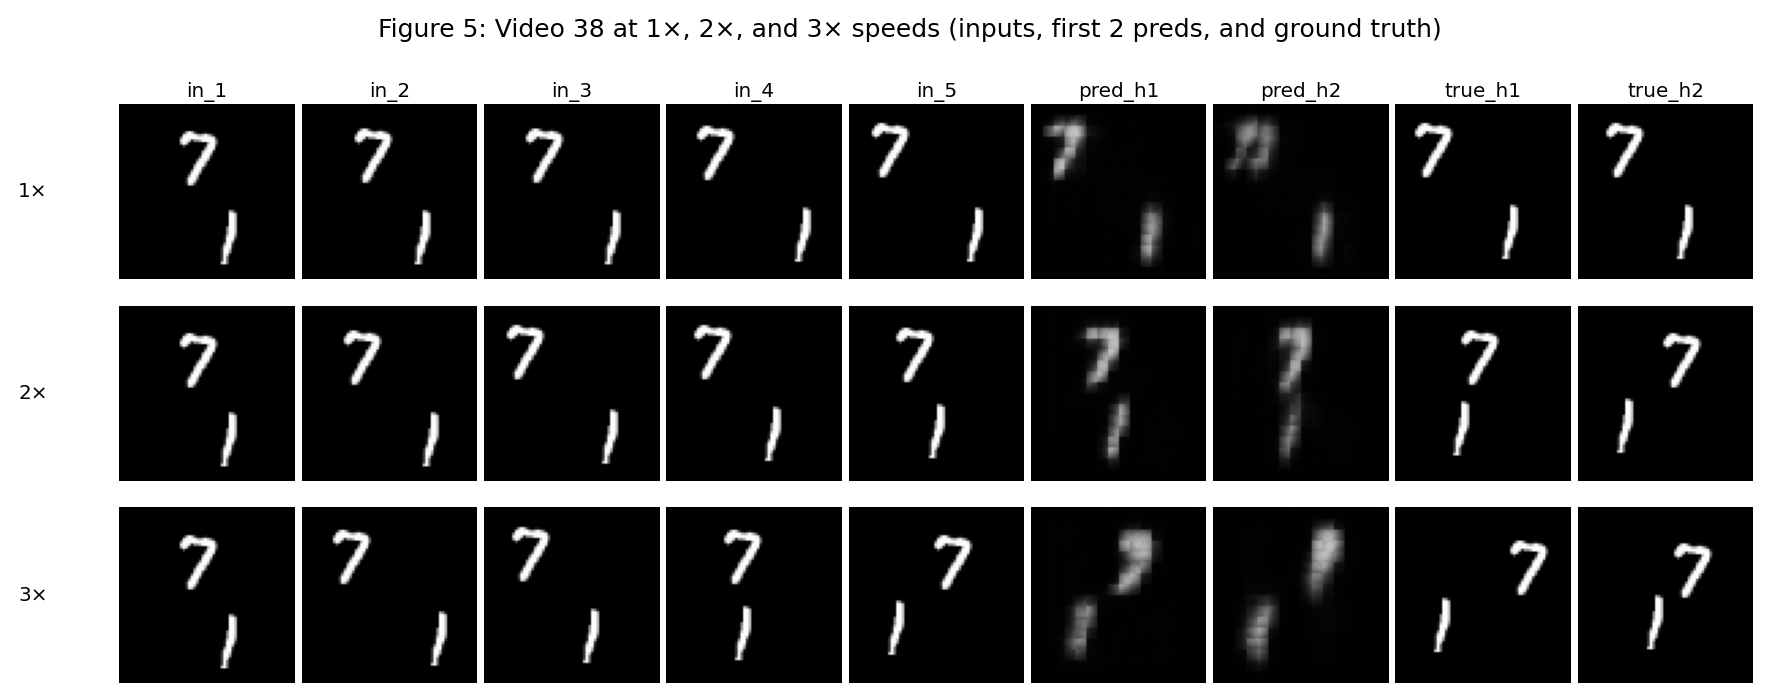
\includegraphics[width=\linewidth]{../Question2/figures/figure5_speeds.png}
\end{minipage}

\q{Q2.9 When does model A fall apart, and does it match the reach?}
\begin{itemize}
  \item At $2\times$: the error jumps from 0.0188 to 0.0447, worse than Blank (0.0425), while $3\times$ adds little (0.0519). This contradicts my estimate, since $2\times$ motion (6.6 px) is within the 8 px reach. Reach only says how far information \emph{can} travel; the weights only learned steps of about 3 px.
  \item In Figure 6, at $2\times$ both digits \textbf{lag} behind and merge into one streak; at $3\times$ they \textbf{stall} near their last positions, the 1's bounce off the wall is missed, and the blobs fade. Lagging and stalling mean it applies its $1\times$ step size; blur means it hedges between possible positions; merging means it does not track nearby digits separately.
\end{itemize}

\q{Q2.10 Unfamiliar motion or reach?} At $3\times$ both causes apply, so model A alone cannot say. At $2\times$ only unfamiliar motion applies. Test: train C (same network, mixed speeds) and D (like C with a larger reach). If C fixes $3\times$, the cause is unfamiliar motion; if only D does, it is reach.

\subsection{4. What Can Data Fix?}

B is A trained on randomly flipped and rotated clips, C is A trained on random speeds ($1\times$ to $3\times$), and D has a larger reach and is trained like C. A check of the training samplers confirmed these rules.

\q{Q2.11 Pre-registered prediction:}
Model B will fix the mirror and rotation failures because it learns to handle flipped and rotated digits, but it won't help at $2\times$ or $3\times$ speed. Model C will improve $2\times$ speed because it is trained on faster motion, but it will still fail at $3\times$, where digits move about 10 px per frame, beyond its 8 px limit. Model D will fix $3\times$ speed because its 16 px reach lets it follow fast-moving digits between frames.

\q{Q2.12 Model D.} Model A with $5 \times 5$ instead of $3 \times 3$ filters, and 46 instead of 64 channels to stay within budget: 709,520 parameters, below the limit of 721,176. A $5 \times 5$ filter passes information 2 cells, so the reach is 4 cells $\times$ 4 px = \textbf{16 px per step}, twice model A's. I chose it before training: designs reaching only 12 px fall short of the fastest $3\times$ motion (14 px), and the other 16 px design would also have changed the image resolution. \textbf{D seed 0 collapsed} into always predicting the same grey frame from epoch 2 (visible on validation); I kept it and report both seeds.

\begin{table}[H]
\caption{Table 7: models A--D (D seed 0 collapsed, so compare D seed 1). Times in seconds}
\centering
\resizebox{\textwidth}{!}{%
\begin{tabular}{lccccccccrcc}
\toprule
Model & $E^{(5)}$ $1\times$ & $C_M$ & $E_M$ & $C_R$ & $E_R$ & $E^{(2)}$ $1\times$ & $E^{(2)}$ $2\times$ & $E^{(2)}$ $3\times$ & Params & Train/epoch & Inference \\
\midrule
A & \ms{0.0222}{0.0225}{0.0219} & \ms{0.00186}{0.00161}{0.00211} & \ms{0.0228}{0.0230}{0.0225} & \ms{0.00298}{0.00268}{0.00329} & \ms{0.0239}{0.0240}{0.0238} & \ms{0.0188}{0.0192}{0.0185} & \ms{0.0447}{0.0435}{0.0459} & \ms{0.0519}{0.0509}{0.0529} & 480,784 & \ms{1.81}{1.86}{1.77} & \ms{0.0609}{0.0608}{0.0609} \\
B & \ms{0.0226}{0.0230}{0.0222} & \ms{0.00123}{0.00117}{0.00128} & \ms{0.0226}{0.0230}{0.0222} & \ms{0.00147}{0.00148}{0.00146} & \ms{0.0224}{0.0228}{0.0221} & \ms{0.0189}{0.0192}{0.0186} & \ms{0.0443}{0.0445}{0.0440} & \ms{0.0509}{0.0509}{0.0509} & 480,784 & \ms{2.01}{2.02}{2.00} & \ms{0.0609}{0.0608}{0.0609} \\
C & \ms{0.0265}{0.0270}{0.0260} & \ms{0.00134}{0.00141}{0.00128} & \ms{0.0267}{0.0272}{0.0262} & \ms{0.00257}{0.00270}{0.00245} & \ms{0.0276}{0.0280}{0.0272} & \ms{0.0231}{0.0237}{0.0225} & \ms{0.0285}{0.0289}{0.0282} & \ms{0.0333}{0.0334}{0.0333} & 480,784 & \ms{1.78}{1.78}{1.77} & \ms{0.0609}{0.0608}{0.0609} \\
D & \ms{0.0336}{0.0401}{0.0271} & \makecell{\sci{6.18}{-4}\\[-2pt]\tiny(\sci{2.68}{-7}, 0.00124)} & \ms{0.0338}{0.0401}{0.0274} & \makecell{0.00119\\[-2pt]\tiny(\sci{6.94}{-7}, 0.00238)} & \ms{0.0342}{0.0401}{0.0284} & \ms{0.0323}{0.0402}{0.0245} & \ms{0.0338}{0.0401}{0.0276} & \ms{0.0355}{0.0402}{0.0308} & 709,520 & \ms{2.01}{2.01}{2.01} & \ms{0.0614}{0.0613}{0.0615} \\
\bottomrule
\end{tabular}}
\end{table}

\q{Q2.13 Label each failure.}
\begin{itemize}
  \item \textbf{Mirror and rotation: appearance.} B changes only how the training digits look, and the error increase disappears ($E_M$ = $E^{(5)}$ = 0.0226) while $C_R$ halves (0.00298 to 0.00147).
  \item \textbf{$2\times$: unfamiliar motion.} C has the same 8 px reach as A but has seen fast motion, and its $2\times$ error drops by 36\% (0.0447 to 0.0285).
  \item \textbf{$3\times$: mostly unfamiliar motion.} C cuts it by 36\% (0.0519 to 0.0333) with no extra reach; D seed 1 gains only a further 8\% (0.0308). So ``C bad, D good'' did not happen. Reach was not a hard wall because a digit is about 20 px wide, so its old and new positions still overlap, a diagonal move is shorter in each direction, and the model's memory carries information across steps.
  \item \textbf{Had C failed and D succeeded,} the limit would be the network itself. Training only tunes the connections that exist; a $3 \times 3$ filter has no connection to cells two steps away, so no amount of data can make information jump further.
\end{itemize}

\q{Q2.14 Did the fixes cost accuracy at $1\times$?} B: no (0.0226 against 0.0222, within the seed spread). C and D: about 20\% worse (0.0265, D seed 1 0.0271), but at $2\times$ and $3\times$ they go from worse than Blank to well below it. Worth it if speeds vary; if only normal speed is expected, A or B is better.

\textbf{How my predictions held up.} Q2.5 was right that rotation is harder than mirroring, but both effects were small, and it was wrong about speed: A broke at $2\times$, not $3\times$. Q2.11 was right about B (except that its gap stayed above zero) and about C at $2\times$, but C also fixed most of $3\times$, and D added only a little.

\subsection{5. The Final Model}

\textbf{Built-in symmetry.} The symmetrised model runs the base model on all 8 flipped and rotated versions of a clip, undoes each transformation and averages. Transforming the input first only reorders those 8 terms, so the output transforms in exactly the same way, whatever the weights: $C_M = C_R = 0$. \textbf{Final model: symmetrised D}, since it is the only model trained for fast motion; D+B was not trained because the wrapper already gives what B's training adds. Figure 7 uses \textbf{seed 1}, because seed 0 collapsed and would show only grey frames.

\begin{table}[H]
\caption{Table 8: symmetrised B and symmetrised D (final model). Training time is that of B and D; inference includes all 8 passes. Times in seconds}
\centering
\resizebox{\textwidth}{!}{%
\begin{tabular}{lccccccccrcc}
\toprule
Model & $E^{(5)}$ $1\times$ & $C_M$ & $E_M$ & $C_R$ & $E_R$ & $E^{(2)}$ $1\times$ & $E^{(2)}$ $2\times$ & $E^{(2)}$ $3\times$ & Params & Train/epoch & Inference \\
\midrule
Sym-B & \ms{0.0219}{0.0223}{0.0216} & \makecell{\sci{4.40}{-17}\\[-2pt]\tiny(\sci{4.72}{-17}, \sci{4.07}{-17})} & \ms{0.0219}{0.0223}{0.0216} & \makecell{\sci{4.51}{-17}\\[-2pt]\tiny(\sci{4.84}{-17}, \sci{4.17}{-17})} & \ms{0.0219}{0.0223}{0.0216} & \ms{0.0184}{0.0186}{0.0182} & \ms{0.0434}{0.0438}{0.0431} & \ms{0.0498}{0.0500}{0.0497} & 480,784 & \ms{2.01}{2.02}{2.00} & \ms{0.253}{0.255}{0.251} \\
Sym-D & \ms{0.0336}{0.0401}{0.0270} & \makecell{\sci{1.61}{-17}\\[-2pt]\tiny(\sci{6.18}{-18}, \sci{2.61}{-17})} & \ms{0.0336}{0.0401}{0.0270} & \makecell{\sci{1.64}{-17}\\[-2pt]\tiny(\sci{5.88}{-18}, \sci{2.68}{-17})} & \ms{0.0336}{0.0401}{0.0270} & \ms{0.0323}{0.0402}{0.0244} & \ms{0.0338}{0.0401}{0.0274} & \ms{0.0354}{0.0402}{0.0306} & 709,520 & \ms{2.01}{2.01}{2.01} & \ms{0.333}{0.337}{0.329} \\
\bottomrule
\end{tabular}}
\end{table}

\begin{figure}[H]
\caption{Figure 7: final model (symmetrised D, seed 1). (a) the Figure 4 videos (GIFs in \texttt{gifs/}); (b) the Figure 6 video}
\centering
\begin{minipage}[c]{0.56\textwidth}\centering
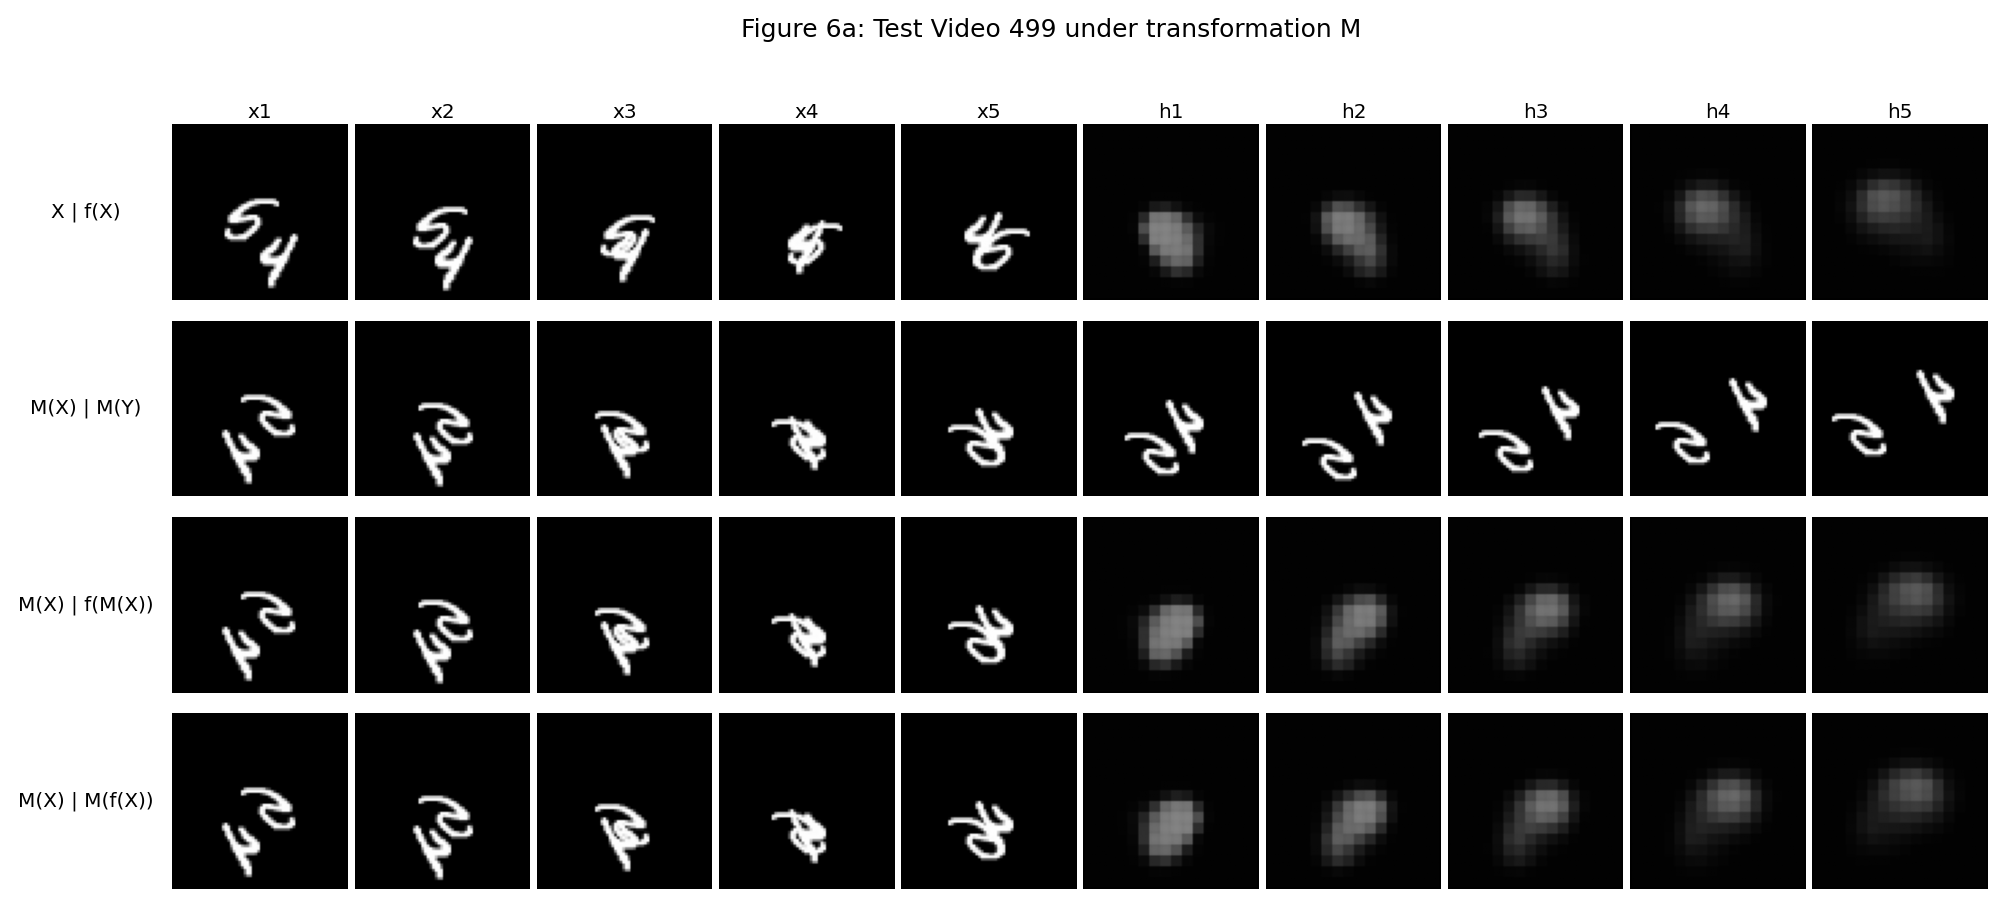
\includegraphics[width=0.49\linewidth]{../Question2/figures/figure6a_M_top1_video499.png}\hfill
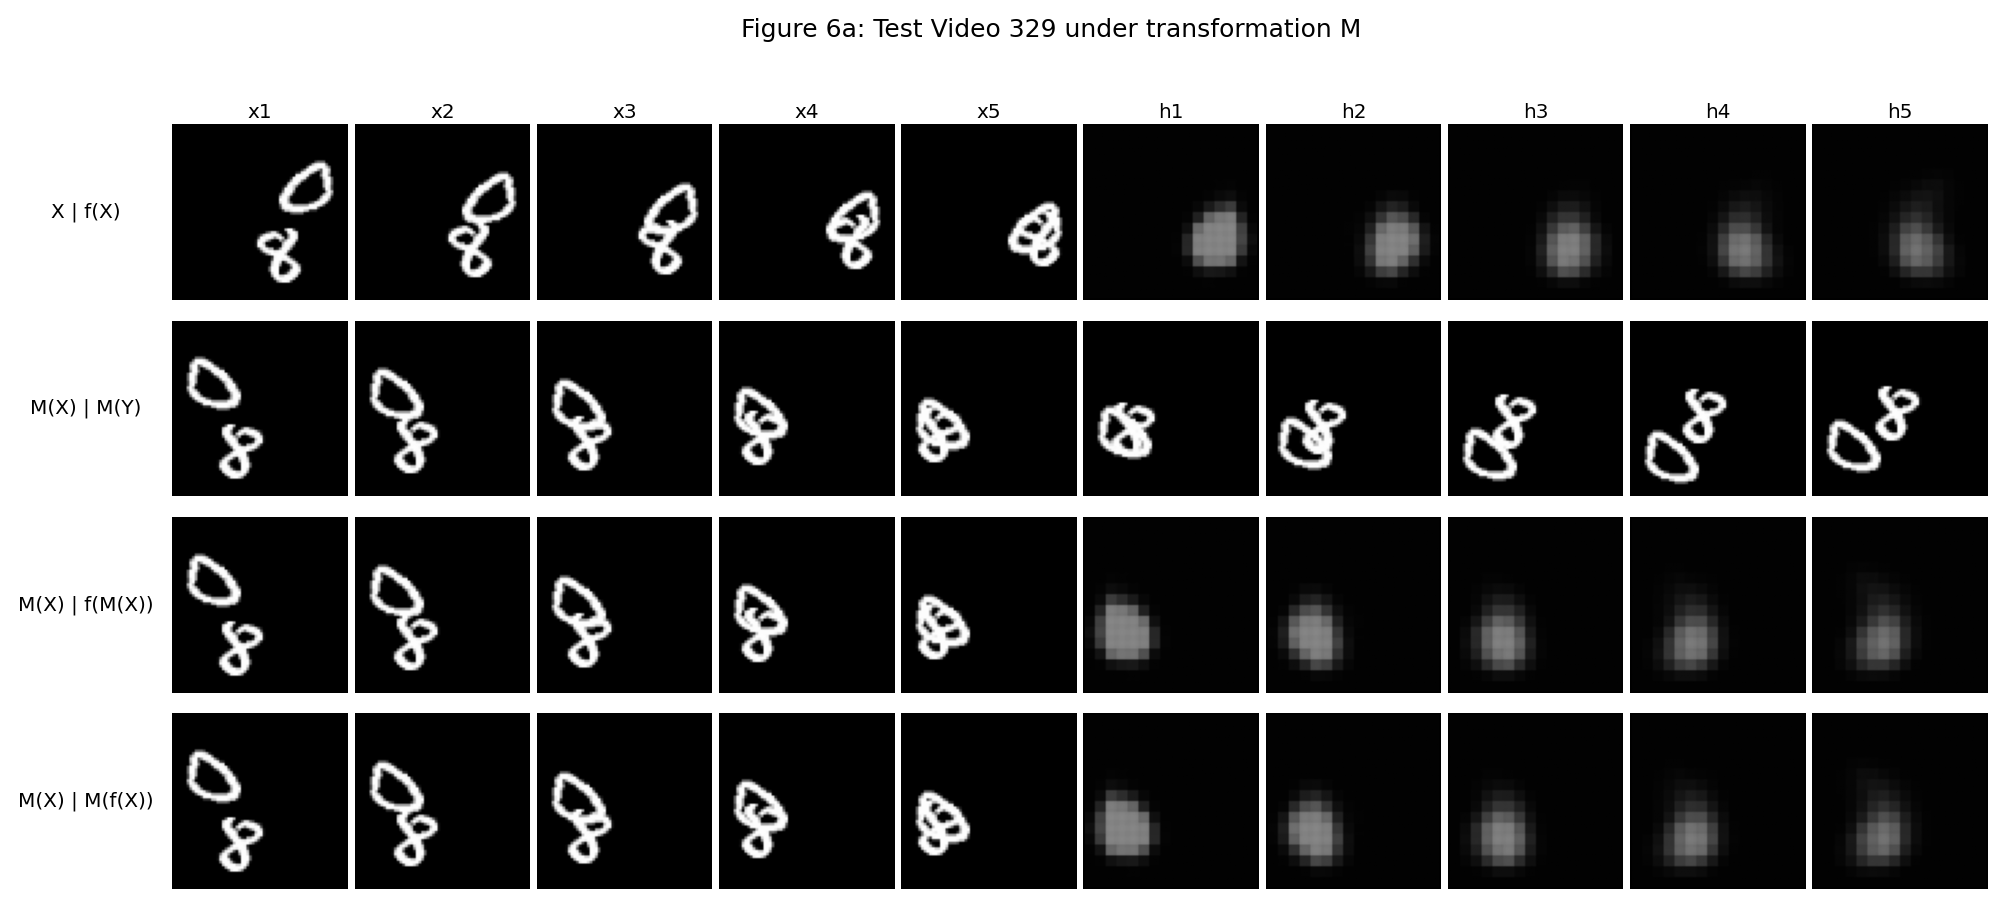
\includegraphics[width=0.49\linewidth]{../Question2/figures/figure6a_M_top2_video329.png}\\[2pt]
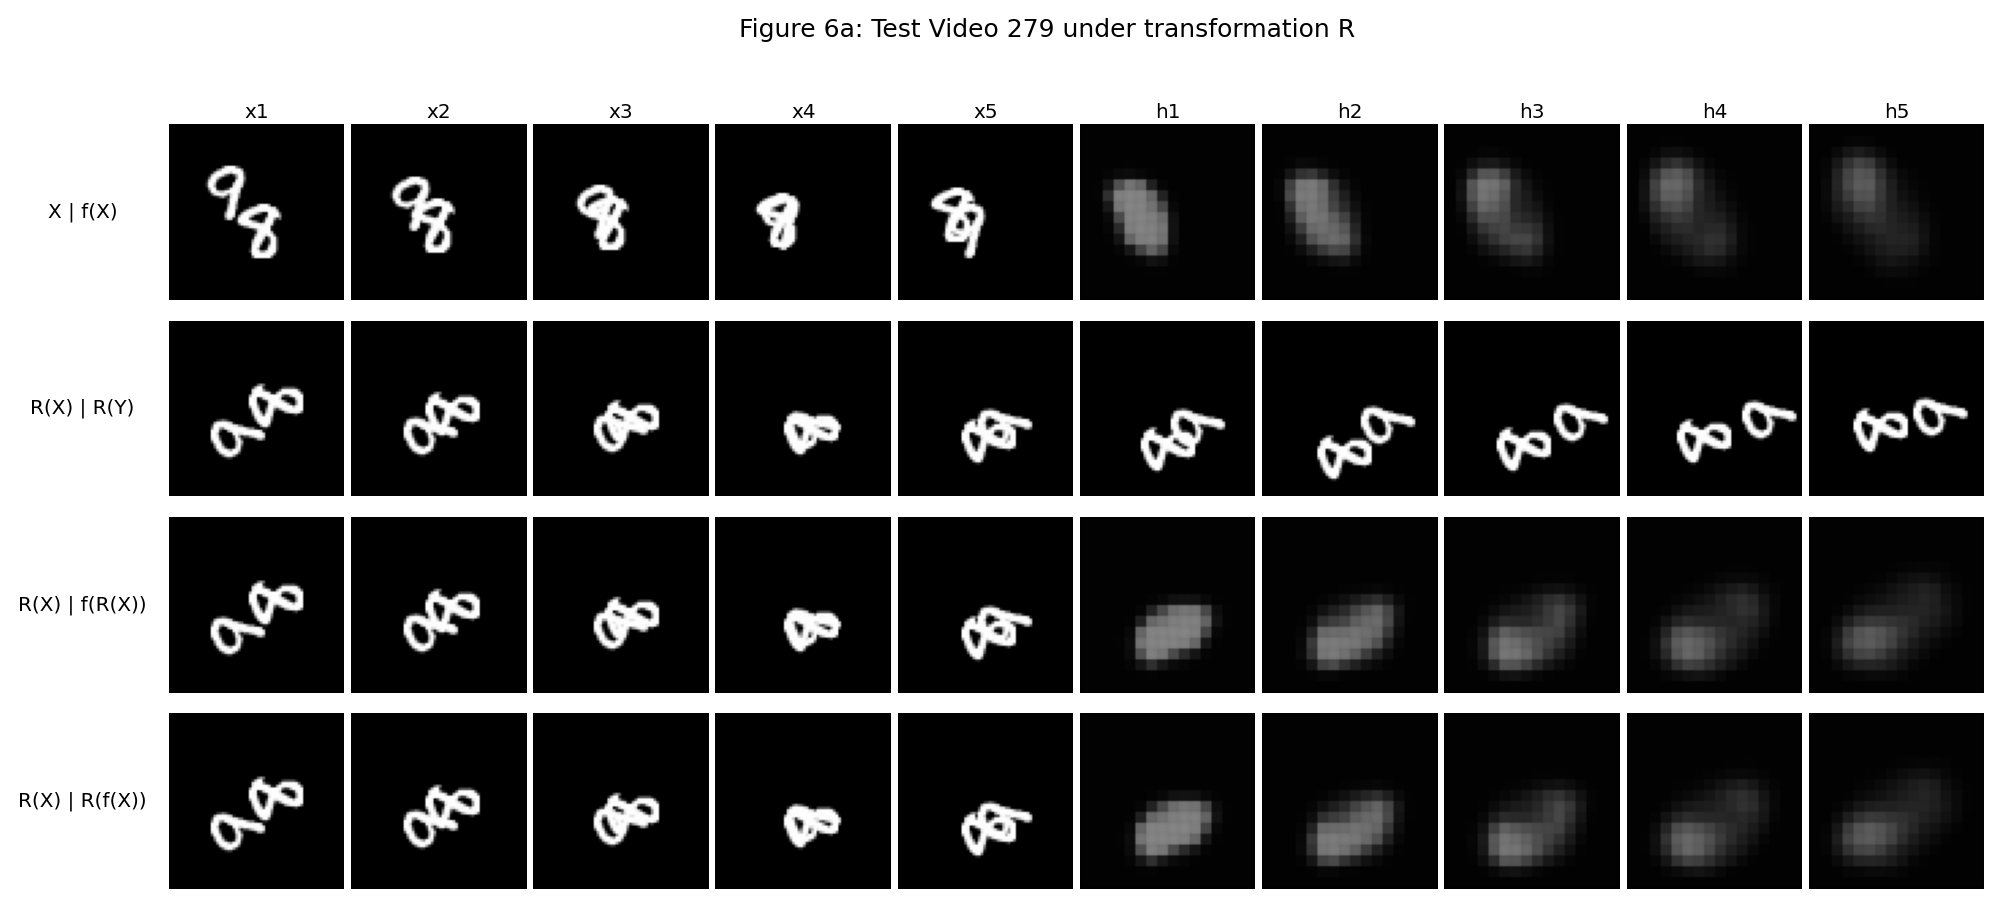
\includegraphics[width=0.49\linewidth]{../Question2/figures/figure6a_R_top1_video279.png}\hfill
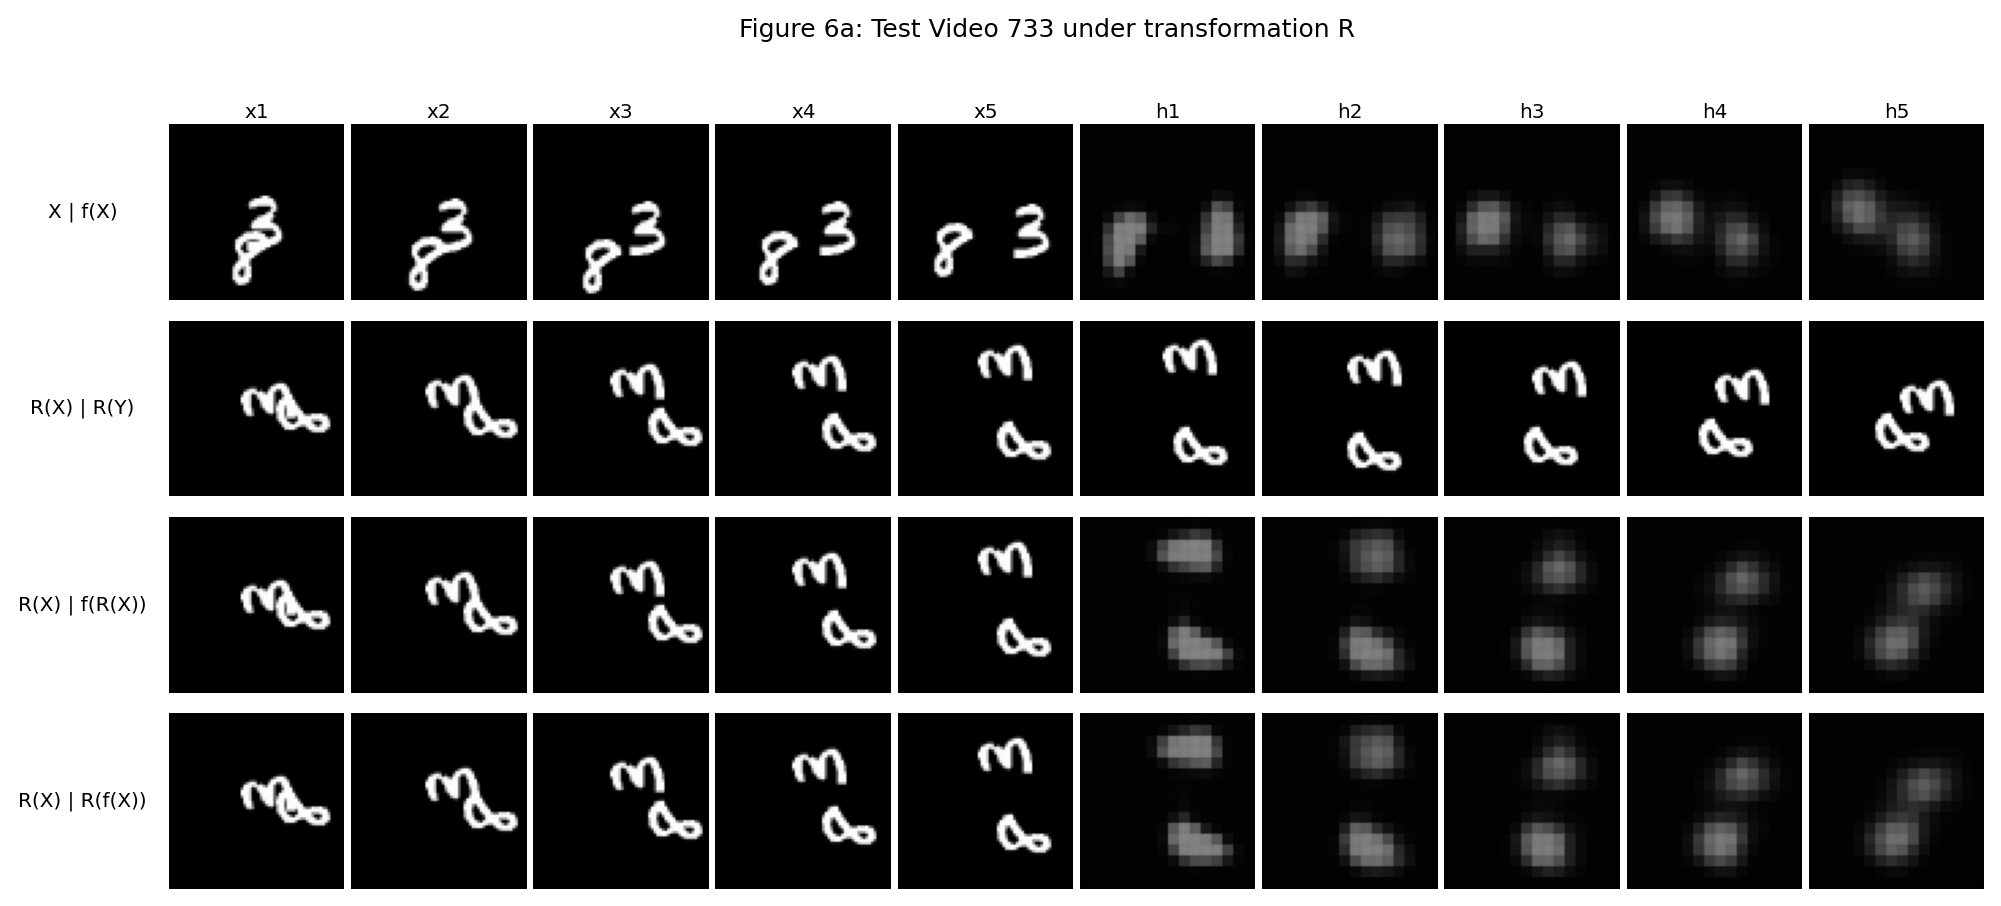
\includegraphics[width=0.49\linewidth]{../Question2/figures/figure6a_R_top2_video733.png}
\end{minipage}\hfill
\begin{minipage}[c]{0.38\textwidth}\centering
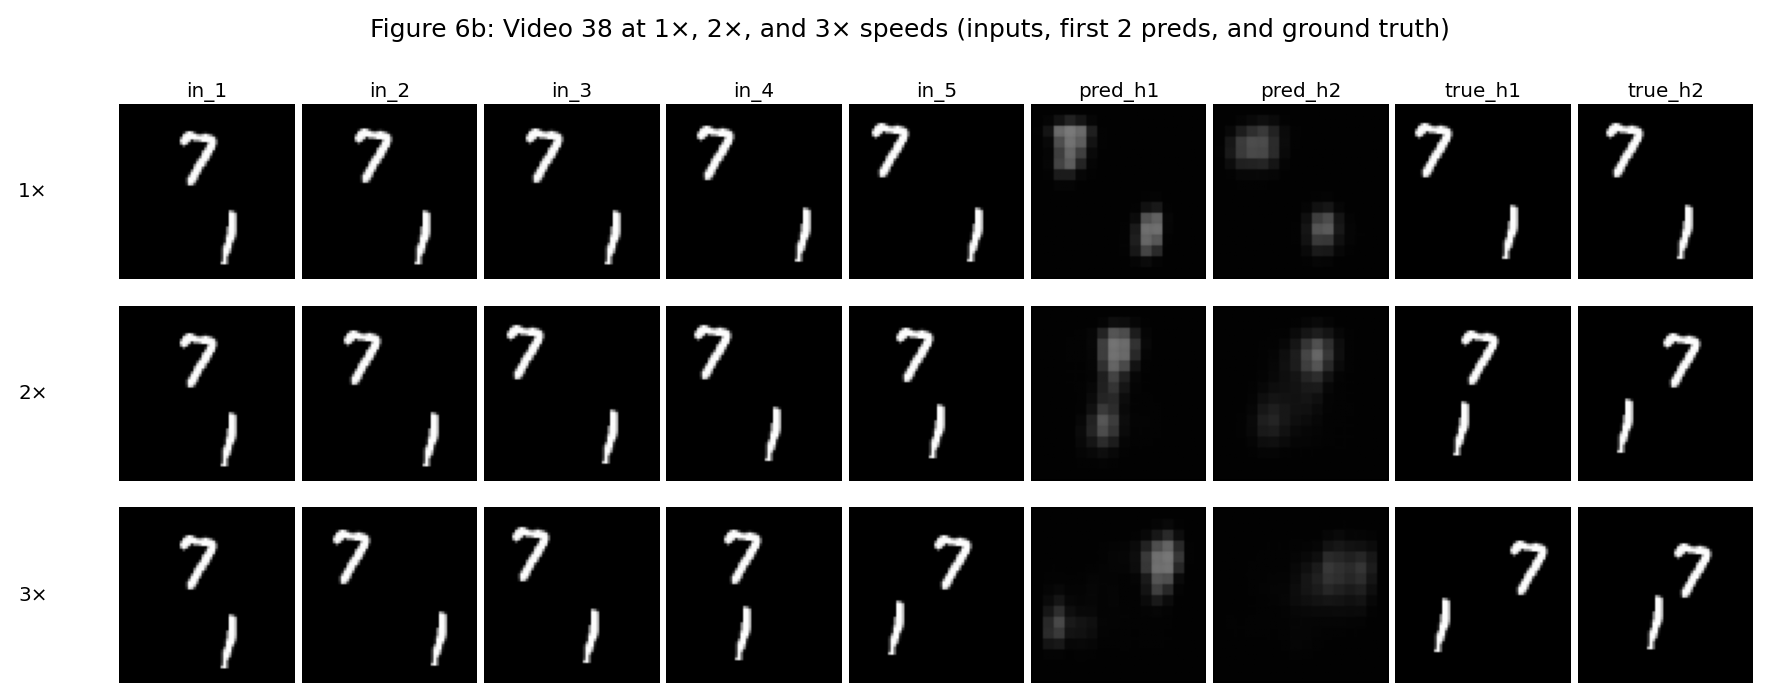
\includegraphics[width=\linewidth]{../Question2/figures/figure6b_speeds_final.png}
\end{minipage}
\end{figure}

\q{Q2.15 Learned (B) or built-in symmetry?}
\begin{itemize}
  \item \textbf{Consistency:} B's gap shrinks but stays (0.00123, 0.00147). The built-in version is exact (about $10^{-17}$, i.e.\ rounding error), guaranteed by construction rather than by training.
  \item \textbf{Accuracy:} averaging helped slightly: Sym-B 0.0219 against B's 0.0226, Sym-D seed 1 0.0270 against 0.0271, and the same at $2\times$ and $3\times$.
  \item \textbf{Cost:} 8 passes per clip made it 4--5 times slower on this GPU (0.253 s against 0.0609 s for B). Learned symmetry costs nothing at prediction time.
  \item \textbf{When it would hurt:} if the 8 predictions were sharp but disagreed, their average would be 8 faint ghosts; or if the data were not symmetric (gravity, readable text). Neither applies here.
\end{itemize}

\q{Q2.16 Video 499 again (Figure 7a).} Rows 3 and 4 are now identical, so the \textbf{symmetrisation} fixed the inconsistency. But the motion is still wrong: the single story it tells is the worse one, a blob following the 4 while the 5 is lost. D's speed training and reach do not matter for this slow clip; they help in Figure 7(b), where at $3\times$ the first prediction places both digits near the truth, unlike model A.

\q{Q2.17 Final verdict.} Partly. The final model learned a rough motion rule, not just what digits look like: mirrored and rotated clips cost it nothing, and its $3\times$ error (0.0306, seed 1) is far below model A's (0.0519) and Blank's (0.0426). But it predicts blurry blobs rather than digits, merges digits that overlap, and one of the two D seeds failed to train. A skeptic would want to see the same rule work on other shapes, over longer horizons, and with both seeds training. One test it still fails: keeping two overlapping digits apart until they separate (video 499).


\section{Attribution and AI usage}

\subsection{Question 1}
I used Mermaid AI to build the architectural diagram based on my notes and knowledge, then used Claude to review and validate it. I used Claude in \texttt{/learn} mode to analyze the requirements of Problem 1 and formulate the proposed design.
\begin{itemize}
\item \textbf{Understanding and design.} Prompts: the assignment zip; ``Let's just focus on Question 1, how can we approach this question?''; ``How can we formulate such problems like architecture from ground up, like token embeddings \dots''; ``SHARE ANSWER''. Output: the per-station approach, the design method (tokens, masked attention, readout) and a worked schedule token. (artifact: \href{https://drive.google.com/file/d/1dPEW6yz6XJP6TbEB3uXsjzDoKoRwyV4H/view?usp=sharing}{River Forecast Design Notes}).
\item \textbf{Study guide.} Prompts: ten questions asked together, from ``What exactly should I predict, and what makes a prediction useful here?'' to ``Put all my decisions together into one clear step-by-step design. Then tell me the weakest parts and what I should test first.'', then ``add some architectural blocks as well''. Output: plain-language answers with block diagrams (artifact: \href{https://drive.google.com/file/d/1p3HH_8zBmhvQWoTHxchM9M3awnjqbeNx/view?usp=sharing}{River Forecast Study Guide}).
\item \textbf{Report.} I first used Claude Opus 5.5 in \texttt{/learn} mode to break down the requirements of Problem 1 and develop my solution. Building on my notes and prior Claude conversations, I then used Claude Opus 5.5 to structure, refine, and finalize the report. Prompts: ``give me summary of first question again \dots''; my Assignment 1 report with ``understand the report writing style and structure, prepare the report for Question 1 \dots''. Output: this report and Figure 1.
\end{itemize}

\subsection{Question 2: Claude and Claude Code}
\begin{itemize}
  \item I used Claude and Claude Code to understand Model A's ConvLSTM architecture and reach, write boilerplate code for the transformation ($M$, $R$) and speed ($2\times$, $3\times$) pipeline, and generate code for Models B--D and the 8-pass symmetrised wrapper (Sym-B, Sym-D).
  \item They helped set up the transformation, gradient-reach, and sampler checks (Table 3, Q2.3), and check Model D ($5 \times 5$ filters, 46 channels) against the reach target and parameter limit before training, using the validation split only to monitor training, and keeping both seeds (including the collapsed D seed 0) rather than tuning on the 1,000 test videos.
  \item I also discussed design choices with them (such as separating unfamiliar motion from reach across C and D), and used them to review code and explain errors.
  \item Claude checked that every number in Tables 3--8 matches the notebook outputs, and I re-ran the full notebook end-to-end so all tables, figures, and GIFs come from one consistent run.
  \item For the report, I used Claude to organise Sections 1--5, understand what each question (Q2.1--Q2.17) was asking, and work through probable answers, which I checked against the plots and tables from the notebook run before finalising.
\end{itemize}

\end{document}
